% \tracingall
% \documentclass[letterpaper]{book}
\documentclass{book}
\usepackage[paperheight=9in,paperwidth=6in,top=1in,bottom=1in,right=1in,left=1in,heightrounded]{geometry}
\usepackage{epsf}
\usepackage{psfig}
\usepackage{palatino}
\usepackage{moreverb}
\usepackage[dvips]{color}
\usepackage{supertabular}
\usepackage{ge}
\title{\Huge\bfseries\sffamily G R A P H I C S \ \ E N G I N E}
\author{\it Lawrence Kesteloot\\\it Rob Wheeler}
\makeindex
\begin{document}
\begin{titlepage}
\setlength{\unitlength}{1in}
\begin{picture}(5,7)(0,0)
\put(0,-1){\epsfbox{emem.ps}}
\put(4.9,7){\makebox(0,0)[rt]{\Huge\scshape\rmfamily G r a p h i c s}}
\put(4.9,6.2){\makebox(0,0)[r]{\Huge\scshape\rmfamily E n g i n e}}
\put(4.9,4){\makebox(0,0)[r]{\large\it Lawrence Kesteloot}}
\put(4.9,3.7){\makebox(0,0)[r]{\large\it Rob Wheeler}}
\put(4.9,0.3){\makebox(0,0)[rb]{\large\scshape Spring 1995}}
\put(4.9,0.0){\makebox(0,0)[rb]{\large\scshape Comp 265 Project}}
\put(5,0){\line(0,1){7}}
\end{picture}
\pagenumbering{roman}
\end{titlepage}
\vspace*{3in}
\noindent Copyright 1995 by Lawrence Kesteloot and Robert Wheeler\par
\vspace{2ex}
\noindent Rambus is a trademark of Rambus, Inc.\par
\noindent FBRAM and 3DRAM are trademarks of Mitsubishi Electric.\par
\vspace{5ex}
\noindent The cover triangle was rasterized by the Graphics Engine's
simulator and the sample application provided in the appendix.
\tableofcontents
\listoffigures
\listoftables

% Define a light gray for box backgrounds:
\definecolor{shadowgray}{gray}{0.7}
\definecolor{unusedgray}{gray}{0.95}

% This command scales the figures:
\setlength{\unitlength}{.6em}

\newcommand{\formatOP}[2]{
{\scriptsize
\begin{picture}(32,4)(0, 0)
\put(.5,-.5){\fboxsep 0pt\colorbox{shadowgray}{\framebox(32,4){}}}
\put(0,0){\fboxsep 0pt\colorbox{white}{\framebox(32,4){}}}
\put(0,0){\framebox(6,4){\shortstack{{#1}\\{\small\tt #2}}}}
\put(6,0){\fboxsep 0pt\colorbox{unusedgray}{\framebox(26,4){\small 0}}}
\put(1,4.9){\makebox(0,0){31}}
\put(5,4.9){\makebox(0,0){26}}
\put(7,4.9){\makebox(0,0){25}}
\put(31.5,4.9){\makebox(0,0){0}}
\put(3,-1.5){\makebox(0,0){6}}
\put(18,-1.5){\makebox(0,0){26}}
\end{picture}
}
}

\newcommand{\formatR}[2]{
{\scriptsize
\begin{picture}(32,4)(0, 0)
\put(.5,-.5){\fboxsep 0pt\colorbox{shadowgray}{\makebox(32,4){}}}
\put(0,0){\fboxsep 0pt\colorbox{white}{\framebox(32,4){}}}
\put(0,0){\framebox(6,4){\shortstack{{#1}\\{\small\tt #2}}}}
\put(6,0){\framebox(5,4){\small r1}}
\put(11,0){\fboxsep 0pt\colorbox{unusedgray}{\framebox(21,4){\small 0}}}
\put(1,4.9){\makebox(0,0){31}}
\put(5,4.9){\makebox(0,0){26}}
\put(7,4.9){\makebox(0,0){25}}
\put(10,4.9){\makebox(0,0){21}}
\put(12,4.9){\makebox(0,0){20}}
\put(31.5,4.9){\makebox(0,0){0}}
\put(3,-1.5){\makebox(0,0){6}}
\put(8.5,-1.5){\makebox(0,0){5}}
\put(21.5,-1.5){\makebox(0,0){21}}
\end{picture}
}
}

\newcommand{\formatRR}[2]{
{\scriptsize
\begin{picture}(32,4)(0, 0)
\put(.5,-.5){\fboxsep 0pt\colorbox{shadowgray}{\makebox(32,4){}}}
\put(0,0){\fboxsep 0pt\colorbox{white}{\framebox(32,4){}}}
\put(0,0){\framebox(6,4){\shortstack{{#1}\\{\small\tt #2}}}}
\put(6,0){\framebox(5,4){\small r1}}
\put(11,0){\framebox(5,4){\small r2}}
\put(16,0){\fboxsep 0pt\colorbox{unusedgray}{\framebox(16,4){\small 0}}}
\put(1,4.9){\makebox(0,0){31}}
\put(5,4.9){\makebox(0,0){26}}
\put(7,4.9){\makebox(0,0){25}}
\put(10,4.9){\makebox(0,0){21}}
\put(12,4.9){\makebox(0,0){20}}
\put(15,4.9){\makebox(0,0){16}}
\put(17,4.9){\makebox(0,0){15}}
\put(31.5,4.9){\makebox(0,0){0}}
\put(3,-1.5){\makebox(0,0){6}}
\put(8.5,-1.5){\makebox(0,0){5}}
\put(13.5,-1.5){\makebox(0,0){5}}
\put(24,-1.5){\makebox(0,0){16}}
\end{picture}
}
}

\newcommand{\formatRRR}[2]{
{\scriptsize
\begin{picture}(32,4)(0, 0)
\put(.5,-.5){\fboxsep 0pt\colorbox{shadowgray}{\makebox(32,4){}}}
\put(0,0){\fboxsep 0pt\colorbox{white}{\framebox(32,4){}}}
\put(0,0){\framebox(6,4){\shortstack{{#1}\\{\small\tt #2}}}}
\put(6,0){\framebox(5,4){\small r1}}
\put(11,0){\framebox(5,4){\small r2}}
\put(16,0){\framebox(5,4){\small r3}}
\put(21,0){\fboxsep 0pt\colorbox{unusedgray}{\framebox(11,4){\small 0}}}
\put(1,4.9){\makebox(0,0){31}}
\put(5,4.9){\makebox(0,0){26}}
\put(7,4.9){\makebox(0,0){25}}
\put(10,4.9){\makebox(0,0){21}}
\put(12,4.9){\makebox(0,0){20}}
\put(15,4.9){\makebox(0,0){16}}
\put(17,4.9){\makebox(0,0){15}}
\put(20,4.9){\makebox(0,0){11}}
\put(22,4.9){\makebox(0,0){10}}
\put(31.5,4.9){\makebox(0,0){0}}
\put(3,-1.5){\makebox(0,0){6}}
\put(8.5,-1.5){\makebox(0,0){5}}
\put(13.5,-1.5){\makebox(0,0){5}}
\put(18.5,-1.5){\makebox(0,0){5}}
\put(26.5,-1.5){\makebox(0,0){11}}
\end{picture}
}
}

\newcommand{\formatRRI}[2]{
{\scriptsize
\begin{picture}(32,4)(0, 0)
\put(.5,-.5){\fboxsep 0pt\colorbox{shadowgray}{\makebox(32,4){}}}
\put(0,0){\fboxsep 0pt\colorbox{white}{\framebox(32,4){}}}
\put(0,0){\framebox(6,4){\shortstack{{#1}\\{\small\tt #2}}}}
\put(6,0){\framebox(5,4){\small r1}}
\put(11,0){\framebox(5,4){\small r2}}
\put(16,0){\framebox(16,4){\small imm}}
\put(1,4.9){\makebox(0,0){31}}
\put(5,4.9){\makebox(0,0){26}}
\put(7,4.9){\makebox(0,0){25}}
\put(10,4.9){\makebox(0,0){21}}
\put(12,4.9){\makebox(0,0){20}}
\put(15,4.9){\makebox(0,0){16}}
\put(17,4.9){\makebox(0,0){15}}
\put(31.5,4.9){\makebox(0,0){0}}
\put(3,-1.5){\makebox(0,0){6}}
\put(8.5,-1.5){\makebox(0,0){5}}
\put(13.5,-1.5){\makebox(0,0){5}}
\put(24,-1.5){\makebox(0,0){16}}
\end{picture}
}
}

\newcommand{\formatRA}[2]{
\formatRRI{#1}{#2}
}

\newcommand{\formatAR}[2]{
\formatRRI{#1}{#2}
}

\newcommand{\formatA}[2]{
{\scriptsize
\begin{picture}(32,4)(0, 0)
\put(.5,-.5){\fboxsep 0pt\colorbox{shadowgray}{\makebox(32,4){}}}
\put(0,0){\fboxsep 0pt\colorbox{white}{\framebox(32,4){}}}
\put(0,0){\framebox(6,4){\shortstack{{#1}\\{\small\tt #2}}}}
\put(6,0){\fboxsep 0pt\colorbox{unusedgray}{\framebox(5,4){\small 0}}}
\put(11,0){\framebox(5,4){\small r2}}
\put(16,0){\framebox(16,4){\small imm}}
\put(1,4.9){\makebox(0,0){31}}
\put(5,4.9){\makebox(0,0){26}}
\put(7,4.9){\makebox(0,0){25}}
\put(10,4.9){\makebox(0,0){21}}
\put(12,4.9){\makebox(0,0){20}}
\put(15,4.9){\makebox(0,0){16}}
\put(17,4.9){\makebox(0,0){15}}
\put(31.5,4.9){\makebox(0,0){0}}
\put(3,-1.5){\makebox(0,0){6}}
\put(8.5,-1.5){\makebox(0,0){5}}
\put(13.5,-1.5){\makebox(0,0){5}}
\put(24,-1.5){\makebox(0,0){16}}
\end{picture}
}
}

\newenvironment{indented}[1]{\vspace{2ex}\noindent{\bf #1}\begin{list}{}{\setlength{\topsep}{0em}}\item}{\end{list}}

\chapter{System Overview}
\pagenumbering{arabic}

\Section{Introduction}
This document outlines the design of the Graphics Engine (GE), which
has an optimized instruction set for transforming and rasterizing 3-D
graphics primitives for low-end machines.  The GE typically is
included in home or arcade video game machines.  A general-purpose CPU
and the GE share memory for communication: The CPU calculates the
game dynamics and sets up a graphics data structure (a display list of
3-D primitives) that the GE traverses and rasterizes in a pipeline
arrangement.  The GE has a RISC core with a back-end specialized
for rasterizing triangles.

A typical application is a game that uses 3-D graphics along with
sound and 2-D sprites (the latter two being supplied by other
hardware).  The application uses the GE to transform, light, and shade
the generated geometry.  A typical game might require up to
3,000 triangles per scene to achieve rendering detail comparable to
current 2-D games.  Thus, at 30 frames a second, roughly 100,000
triangles per second must be transformed and half of these must be lit
and rasterized.  (Over half of the triangles will be removed by
backface and frustum culling.)

The GE instruction set is optimized for the following tasks:
\begin{enumerate}
\item traversing a hierarchical display list;
\item transforming coordinates;
\item calculating plane equations; and
\item rasterizing polygons.
\end{enumerate}
Only minimal 3-D features are supported---clipping,
diffuse lighting, gouraud shading, screen-door transparency, and
Z-buffering.  The GE has no anti-aliasing, texturing, or blending
support.

This is a very specialized CPU, not only because it is optimized
for graphics, but because it is designed for low-end, inexpensive
graphics.  It does not provide the flexibility of high-end graphics
workstations, and the game programmer is expected to abide by
restrictions, such as keeping coordinates within the range of
fixed-point values.  When necessary, we simplified the hardware at the
expense of a heavier burden on the programmer.  Most game programmers
are used to programming in assembler and having no programming support
whatsoever, so these are not unusual nor unexpected demands.

\begin{figure}
\setlength{\unitlength}{1em}
\center{\begin{picture}(28,16)(0,0)
\put(0.5,9.5){\fboxsep 0pt\colorbox{shadowgray}{\makebox(8,5){}}}
\put(10.5,9.5){\fboxsep 0pt\colorbox{shadowgray}{\makebox(8,5){}}}
\put(20.5,9.5){\fboxsep 0pt\colorbox{shadowgray}{\makebox(8,5){}}}
\put(10.5,0.5){\fboxsep 0pt\colorbox{shadowgray}{\makebox(8,5){}}}
%
\put(0,10){\fboxsep 0pt\colorbox{white}{\framebox(8,5){CPU}}}
\put(10,10){\fboxsep 0pt\colorbox{white}{\framebox(8,5){GE}}}
\put(20,10){\fboxsep 0pt\colorbox{white}{\framebox(8,5){Video Hardware}}}
\put(10,1){\fboxsep 0pt\colorbox{white}{\framebox(8,5){RAM}}}
%
\put(4,10){\line(0,-1){2}}
\put(14,10){\line(0,-1){2}}
\put(24,10){\line(0,-1){2}}
\put(14,8){\line(0,-1){2}}
\put(4,8){\line(1,0){20}}
\end{picture}}
\caption{Typical machine configuration}
\label{fig:configuration}
\end{figure}

A typical machine configuration is shown in Figure~\ref{fig:configuration}.
The CPU and the GE will communication via display lists
stored in shared memory.  The CPU will setup the display list for the
next frame while the GE will traverse and rasterize the display list for
the current frame.  Semaphores in memory will keep the producer-consumer
pipeline synchronized.

{\em A note about this architecture document:\/} In a very low-end
high-performance architecture, the application, the processor
architecture, and the implementation are more interdependent than a
pure, transparent architecture will allow.  On the GE in particular, we
not only know what {\em kind\/} of application will run on it, but we
know the actual application!  (Although game writers are free to rewrite
the program running on the GE, most are likely to use the one supplied
in the Appendix of this document.)  As a result, this document describes
the application, the architecture, and touches on the implementation.
In a sense, the application can be seen as part of the architecture,
with the display list being the architecture's machine language and the
on-chip program being the microcode.  In any case, the close synergy
between the three parts of the Graphics Engine allow for a design that
optimizes for both performance and economy.

\Section{Application Background}

In a typical graphics pipeline, geometry (usually triangles) is generated
in 3-D space.  The vertices are transformed by a model-view matrix which
converts the primitives from object space to world space and from world
space to camera space in one step.  The primitives are then lit in
world space, transformed by a projection matrix, clipped to the viewing
frustum, projected onto a 2-D screen, and rasterized (drawn).  See
\cite{foley} for a more complete description of the pipeline.

As is often done in interactive graphics, our pipeline makes some
approximations to reduce the computational burnen on the system.
For example, if we assume that the viewer and the light sources are
infinitely far away, then we can keep a combined model-view-projection
matrix, saving one matrix multiplication.  The normals do not need
to be transformed by the inverse transpose of the model-view matrix
(as would normally be correct); instead, we can transform the light
source and view vectors by the inverse of the model-view matrix,
yielding the same results and saving a matrix multiplication per
vertex.

The rasterization entails finding the area on the screen which is
covered by the primitive and interpolating the information at the
vertices (in our case, color and Z).  We use the \index{plane equation
method}{\em plane-equation\/} method of rasterization.  The idea is that
each edge of a triangle can be described by a equation of the form $Ax
+ By + C = 0$.  Substituting the coordinates of each pixel in the
bounding box of the triangle into all three edge equations will
determine if the pixel is inside or outside the triangle.  Those that
are inside can interpolate parameters using more plane equations of
the form $p = Ax + By + C$, where $p$ is the parameter to be
interpolated.  This method is easier to implement than traditional
edge-walkers, is more easily parallelized, and is often faster for
small triangles\footnote{Although the inside loops of edge-walkers are
tighter than those of plane-equation algorithms, the per-primitive and
per-scanline overhead is not sufficiently amortized on small
triangles.}.

In order for primitives to occlude other primitives that are behind
them, we keep track of the distance to the closest primitive at each
pixel.  This \index{Z-buffer}{\em Z-buffer\/} is initialized to infinity
and for each pixel about to be drawn the Z value in the Z-buffer is
compared to the primitive's Z value at that pixel, and the closest
pixel (the one with the lowest Z value) is placed in the color and Z
buffers.  The Graphics Engine supports a Z-buffer with 16 bits per
pixel, which is certainly enough for game applications and probably
enough for most applications as well\footnote{Although most systems
use from 24 to 32 bits of Z per pixel, much of that resolution (probably
around 8 bits) is lost because of the exponential distribution of Z
values as the yon plane is approached.}.

Since we use hierarchical display lists, a model-view matrix stack is kept
that allows sub-lists' transformations to remain localized.
\index{lighting}Although
in our implementation only diffuse lighting is implemented, the
architecture of the Graphics Engine would support specular
\index{lighting!Phong}(Phong) lighting quite well.

\index{transparency!screen-door}{\em Screen-door transparency\/} is a
method to simulate transparent surfaces by only drawing a subset
of the primitive's pixels, thus allowing the background to show
through.  The GE supports basic screen-door transparency by allowing
a bitmask for each row of 16-pixel inside the primitive.

\Section{System Requirements}

\subsection{Transformation/Rasterization Rate}

If our goal is to draw 100,000 meshed triangled per second, and if we
assume that a simple RISC architecture can easily be run at a 100 MHz
clock rate, then we must transform, light, clip, and rasterize a
triangle in 1000 clock cycles (or almost equivalently, instructions).
If we consider an ``average'' triangle be cover 50 pixels, then a
general-purpose RISC architecture could spend its 1000 instructions
on the rasterization alone!  Clearly, special-purpose instructions
and hardware are needed to achieve our goal.

A more detailed outline of the operations performed per triangle will
show which instructions need attention:

\begin{enumerate}
\item Copy vertex information into buffer.
\item Transform vertex by model-view-projection matrix.
\item Light the vertex.
\item Clip to hither and yon planes.
\item Do perspective divide.
\item Compute screen-space bounding box.
\item Compute edge equations (3).
\item Compute parameter equations (4).
\item Loop over bounding box and rasterize.
\end{enumerate}

Transforming a vertex is an expensive operations, with 16 multiplications
and 12 additions.  A special-purpose dot-product operation is provided
to reduce the time to the equivalent of 4 multiplications and 8 additions.
(Equally significant is that the dot-product operation works directly in
data memory, avoiding the 16 loads that would be required to load the
matrix.)
Lighting also requires a few dot products, and the same dot-product
operation can be used to speed up this part of the pipeline.

Clipping is straightforward and inexpensive (since we only have two
planes to clip to), and normal arithmetic operations can be used.
The perspective divide requires a reciprocal, and since a reciprocal
can be found almost as fast in software as in hardware, a reciprocal
operation is not provided.

Computing the edge and parameter equations requires heavy use of
fixed-point data types, and a fixed-point multiply is provided (in
addition to the integer multiply) to avoid the considerable extra
work that would be required to simulate such an operation in
software.

All of the gains of the above operations, however, could easily be
shadowed by the expensive rasterization loop.  This is where
special-purpose instructions and hardware are most necessary.  We use
a linear-expression tree to allow 16 instances of the linear equations
to be evaluated in 4 clock cycles.  This allows 16 pixels to be tested
against the edge equations and have their parameters interpolated in
about 13 clock cycles.  An average triangle (50 pixels) can be
rasterized in about 400 clock cycles this way, allowing us to reach
our goal.

\subsection{Shared Memory Size}

\noindent{\bf Video memory.}\quad Video memory is {\em
double-buffered}.  Since the output device of this machine is likely
to be an NTSC television or a monitor of comparable quality (in video
arcades), a frame resolution of at most $640\times480$ is required. 
Such a low resolution will increase the effective rasterization speed
since triangles will be smaller.  A colormap system is not acceptable
since we need to interpolate color for lighting\footnote{Internally,
all colors are kept in RGB format.  The architecture does not restrict
the implementation from dithering the final RGB value and using a
colormap system in the frame buffer.}, so an RGB scheme with 5 bits
for red and blue and 6 bits for green is used\footnote{The extra bit
is given to green because the eye is most sensitive to the green part
of the spectrum.  An extra bit will allow more subtle shades of
intensity.}.  A {\em Z-buffer\/} is used for hidden surface removal,
with 16 bits per pixel.  The total video memory requirement is then
$3\mbox{ buffers}\times640\mbox{ X-resolution}\times480\mbox{
Y-resolution}\times2\mbox{ bytes/pixel} = 1,843,200$ bytes.

\vspace{1ex}\noindent{\bf Display list memory.}\quad Each vertex needs
to store three coordinates (x, y, z) of 16 bits each (6 bytes), a
vertex number, and the vertex op-code.
We expect to rasterize about 3,000 triangles per frame, with many of
those in mesh format (one vertex per triangle).  This will take
roughly $6000 \times 8$ bytes plus other information, such as transformation
matrices (which are few).  The total display list memory requirement
is then at most 100,000 bytes per display list, times two since
display lists are double-buffered\footnote{See Section~\ref{sec:dblbuffer}
for a discussion of how to single-buffer most of the display list.}.
The GE will access all memory in big-endian order, so it would be most
efficient if the CPU's endianess were the same.

\vspace{1ex}\noindent{\bf Program memory.}\quad The program running on
the GE will be on-chip. Programs running on the CPU will probably be
at most be 100,000 bytes, plus 200,000 bytes for data.

\vspace{1ex}\noindent{\bf Total.}\quad The total external memory
requirements are then $1.8 + 0.2 + 0.3 = 2.3$ megabytes.  This
probably will be rounded up to 4 megabytes, requiring at least 22 bits
in address fields.

\chapter{Graphics Engine Architecture}

The Graphics Engine is a Harvard architecture chip with 1024 32-bit
words of on-chip program memory, 1024 words of on-chip data memory,
access to external RAM (through DMA, or {\em Direct Memory Access}),
32 word-length registers, one program counter, one status word, and a
RISC instruction set specialized for graphics processing.  It has no
interrupts, exceptions, no memory management unit, and no cache.  See
Figure~\ref{fig:progmodel} for the basic programming model.

\begin{indented}{\bf Operation:}\vspace{.8ex}
\begin{verbatimtab}
typedef unsigned long Word;
\end{verbatimtab}
\end{indented}

\begin{figure}
{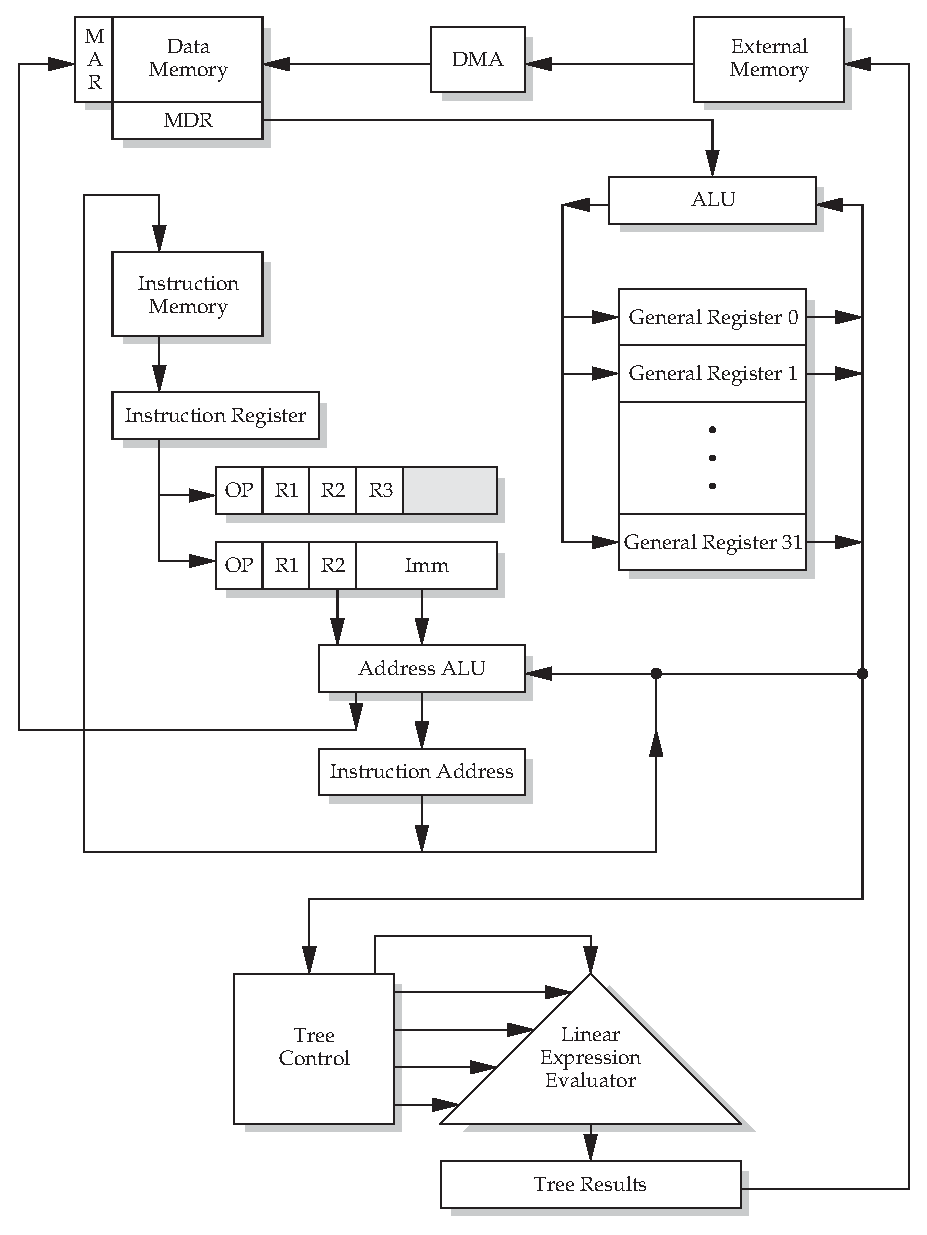
\psfig{file=ge.model.ps,height=6.5in}}
\caption{\label{fig:progmodel}Basic Programming Model}
\end{figure}

\Section{\index{registers}Registers}

The GE has 32 general-purpose registers that are word-length (32 bits).
Reading register 0 always returns 0 and writing to it has no effect.

\begin{indented}{\bf Operation:}\vspace{.8ex}
\begin{verbatimtab}
Word reg[32];
\end{verbatimtab}
\end{indented}

\Section{\index{address space}Address Space}

Memory locations 0 through 1023 address words in the on-chip data
memory.  External RAM is read and written through special DMA
instructions that copy blocks of memory in and out of internal data
memory.  Video memory is accessed through special rasterization
instructions.  There is no direct access to the program counter or the
status word.

\begin{indented}{\bf Operation:}\vspace{.8ex}
\begin{verbatimtab}
Word iMem[1024], dMem[1024], eMem[1 << 22];
\end{verbatimtab}
\end{indented}

\Section{\index{status word}Status Word}

The status word is not bit addressable, but its contents can be tested
with various branching instructions.

\begin{indented}{\sc Bit 0 --- Zero (Z)}
  \begin{itemize}
    \item[If 0] the last arithmetic or logical scalar or vector
          instruction returned a non-zero number.
    \item[If 1] otherwise.
  \end{itemize}
\end{indented}
\begin{indented}{\sc Bit 1 --- Negative (N)}
Set to the most significant bit of the result
of the last arithmetic or logical scalar or vector operation.
\end{indented}

\vspace{1ex}

\noindent The ``Operation'' sections of the instruction descriptions in
Chapter~\ref{chap:instset} use the following function to
set the status word after arithmetic and logical operations:

\begin{indented}{\bf Operation:}\vspace{.8ex}
\begin{verbatimtab}
#define Z 1
#define N 2
Word sw;
SetStatusWord (Word val) {
    nbit = (val >> 31);
    zbit = (val == 0);
    sw = zbit | (nbit << 1);
}
\end{verbatimtab}
\end{indented}

\Section{\index{instruction format}Instruction Format}

There are only two basic instruction formats: RRR and RRI.  The four others
are subsets of one of these.  Six bits are reserved for the op-code,
with the rest reserved for register operands and immediate values.

The OP format only has the op-code.  It is useful for tree instructions
that need no operands.

\vspace{3ex}
\formatOP{000000}{OP}

\vspace{3ex}
The R, RR, and RRR instructions deal with registers directly.  They are
used for arithmetic and logical operations, as well as tree operations.
The R format is not used in the current instruction set.

\vspace{3ex}
\formatR{000001}{R}

\vspace{3ex}
\vspace{3ex}
\formatRR{000002}{RR}

\vspace{3ex}
\vspace{3ex}
\formatRRR{000003}{RRR}

\vspace{2ex}
The RRI format is used both for the immediate logical instructions as well
as for loads and stores.  For the former, the immediate value determines
the number of bits to shift, and for the latter, the second register and
the immediate determine the address to access.

\vspace{3ex}
\formatRRI{000004}{RRI}

\vspace{3ex}
Finally, the A format is used for branches and jumps.  Only the second
register and the immediate are used to determine the branch
destination.  The immediate, being 16 bits, has enough range to cover
the internal instruction space, but the register can optionally be
used for jump tables.  Notice that the assembly language format for
the {\tt LD} and {\tt ST} instructions are reversed: The destination
is always first, even if in the encoding the destination is second
(as in the {\tt ST} instruction).

\vspace{3ex}
\formatA{000005}{A}

\vspace{3ex}

\begin{indented}{\bf Operation:}\vspace{.8ex}
\begin{verbatimtab}
Word pc, inst, op, r1, r2, r3, imm;
inst = iMem[pc++];
op = inst >> 26;
r1 = (inst >> 21) & 0x31;
r2 = (inst >> 16) & 0x31;
r3 = (inst >> 11) & 0x31;
/* Sign-extend immediate: */
imm = (signed long)(signed short)(inst & 0xFFFF);
\end{verbatimtab}
\end{indented}

\vspace{2ex}
\Section{\index{addressing modes}Addressing Modes}

Only the load, store, branch, and jump instructions need to reference
memory.  The first two address internal data memory and the last
two address instruction memory.  All four instruction types add
the second register specified in the instruction word with the immediate
value to determine the address.  Register {\tt R0}, which is always zero,
can be used if the immediate value directly specifies the address.

Notice that the {\tt LI} (Load Immediate) instruction has the same format
as the above four instruction types, but the sum of the second register
and the immediate is placed directly into the first register without
referencing memory, so it is not strictly an addressing mode since
the resulting value is not checked against the memory bounds.

All addresses reference words.  There are no addressing modes for
half-words or bytes.

\begin{indented}{\bf Operation:}\vspace{.8ex}
\begin{verbatimtab}
Word addr;
addr = reg[r2] + imm;
\end{verbatimtab}
\end{indented}

\Section{Rasterization Registers}

The rasterization back-end has several registers that can be set with
the {\tt SCRSET} and {\tt TREESET} instructions.

\begin{indented}{\bf Operation:}\vspace{.8ex}
\begin{verbatimtab}
Word width, height;	/* Size of the screen */
Word fbAddr, zAddr;	/* Location in bytes of buffers */
Word xTree, yTree;	/* Position of left-most pixel of tree */
\end{verbatimtab}
\end{indented}

\Section{Instruction Sequencing}

The instruction set has one unconditional jump and conditional
branches for the following conditions: equal to, not equal to, less
than, less than or equal to, greater than, and greater than or equal
to.  The implementation can assume that these conditional branches are
not likely to be taken.  A ``likely'' version of each branch
instruction is available that allows the implementation to fill the
instruction pipeline from the destination address.  All jump and
branch instructions have their destination address specified by the
sum of a register-immediate pair.  The register can be {\tt R0} (which
is always zero) for absolute addresses.

There is a single branch delay slot which is always executed, whether
or not the branch is taken.  This slot may not be filled with another
branch, jump, or call instruction, although this is not policed and
the results of doing so are undefined.

The processor has no mechanism for halting or termination.  The
application is a loop that continuously reads data from the main CPU
and rasterizes it.

\Section{External Synchronization}

The two DMA instructions {\tt READ} and {\tt WRITE} can read or write
16 words to external memory.  Since the main CPU and the graphics
engine are set up in a typical producer-consumer relationship, two
semaphores (one each way) need to be kept.  The two DMA instructions
can be used for this purpose since there are no race conditions
between the processors.

The {\tt READ} instruction is primarily used to read the display
lists.  The {\tt WRITE} instruction can be used to modify the frame
buffer or to return debugging and performance information to the CPU.

\Section{Policing}

Policing is useful both to facilitate compatibility with future
architectures and to help find bugs.  It is difficult to police an
architecture that has no interrupts or exceptions, so this
architecture tries to at least achieve the first advantage of
policing: A violation halts the processor.  This encourages
programmers to use valid opcodes and to keep memory references in
range.  An exception would have made debugging easier at the cost of
considerable architecture and implementation complications.  (Consider
what happens in the instruction pipeline when an instruction needs to
be restarted after an exception.)  In addition, programmers can use the
simulator to find bugs.

The following violations halt the processor: Invalid op-code; invalid
program counter; invalid data memory reference; invalid tree setup
operands; and DMA access that reads or writes outside of data memory.

\chapter{\index{instruction set}\label{chap:instset}Instruction Set}

Instructions are in the general format
{\tt OP {\em dest},{\em src1},{\em src2}}.  The operands are almost
always registers, and the destination register is allowed to be
the same as one of the source registers.  Almost all operations
set the status bits based on the result of the operation.  Note
that the bits are set before the result is placed in the register.
This means that using {\tt R0} (which is always zero) as a destination
still sets the status bits according to the result of the operation.
Table~\ref{tab:instsummary} on page~\pageref{tab:instsummary} summarizes
the instruction set.

\begin{table}[ht]\small
\begin{tabular}{llll}
Instruction & Operands & Format & Description\\\hline
\tt LD&\tt r1, r2(imm)&RA&Load Register\\
\tt ST&\tt r2(imm), r1&AR&Save Register\\
\tt LI&\tt r1, r2(imm)&RA&Load immediate\medskip\\
\tt ADD&\tt r1, r2, r3&RRR&Fixed-point Add\\
\tt SUB&\tt r1, r2, r3&RRR&Fixed-point Subtract\\
\tt MUL&\tt r1, r2, r3&RRR&Integer Signed Multiplication\\
\tt MULF&\tt r1, r2, r3&RRR&Fixed-point Signed Multiplication\\
\tt RECP&\tt r1, r2&RR&Fixed-point Signed Reciprocal\\
\tt AND&\tt r1, r2, r3&RRR&Bit-wise And\\
\tt OR&\tt r1, r2, r3&RRR&Bit-wise Or\\
\tt XOR&\tt r1, r2, r3&RRR&Bit-wise Xor\\
\tt NOT&\tt r1, r2&RR&Bit-wise Not\\
\tt LSL&\tt r1, r2, r3&RRR&Logical Shift Left\\
\tt LSR&\tt r1, r2, r3&RRR&Logical Shift Right\\
\tt ASR&\tt r1, r2, r3&RRR&Arithmetic Shift Right\\
\tt LSLI&\tt r1, r2, imm&RRI&Logical Shift Left Immediate\\
\tt LSRI&\tt r1, r2, imm&RRI&Logical Shift Right Immediate\\
\tt ASRI&\tt r1, r2, imm&RRI&Arithmetic Shift Right Immediate\medskip\\
\tt JMP&\tt r2(imm)&A&Unconditional Jump\\
\tt CALL&\tt r2(imm)&A&Unconditional Subroutine Call\\
\tt JEQ&\tt r2(imm)&A&Jump If Equal\\
\tt JEQL&\tt r2(imm)&A&Jump If Equal Likely\\
\tt JNE&\tt r2(imm)&A&Jump If Not Equal\\
\tt JNEL&\tt r2(imm)&A&Jump If Not Equal Likely\\
\tt JLT&\tt r2(imm)&A&Jump If Less Than\\
\tt JLTL&\tt r2(imm)&A&Jump If Less Than Likely\\
\tt JLE&\tt r2(imm)&A&Jump If Less Than or Equal To\\
\tt JLEL&\tt r2(imm)&A&Jump If Less Than or Equal To Likely\\
\tt JGT&\tt r2(imm)&A&Jump If Greater Than\\
\tt JGTL&\tt r2(imm)&A&Jump If Greater Than Likely\\
\tt JGE&\tt r2(imm)&A&Jump If Greater Than or Equal To\\
\tt JGEL&\tt r2(imm)&A&Jump If Greater Than or Equal To Likely\medskip\\
\tt DOT&\tt r1, r2, r3&RRR&Fixed-point Vector Dot-Product\medskip\\
\tt READ&\tt r1, r2&RR&DMA Read from External Memory\\
\tt WRITE&\tt r1, r2&RR&DMA Write to External Memory\medskip\\
\tt SCRSET&\tt r1, r2, imm&RRI&Set Screen Location\\
\tt CLS&\tt r1, r2&RR&Clear Screen\\
\tt TREESET&\tt r1, r2, r3&RRR&Setup Tree and Clear Enable Flags\\
\tt TREEIN&\tt r1, r2&RR&Edge Equation Test\\
\tt TREEVAL&\tt r1, r2, imm&RRI&Parameter Interpolation\\
\tt TREEPUT&\tt &OP&Tree Write to Frame Buffer\\
\end{tabular}
\caption{Instruction Set Summary}
\label{tab:instsummary}
\end{table}

\Section{Register Loading and Storing}
\noindent\textsf{\textbf{\Large LD}}\index{instruction set!LD@{\tt LD}}\par
\noindent {\sc Load Register}\par\begin{indented}{\bf Format:}
{\tt LD r1, r2(imm)}\par\vspace{3ex}
\formatRA{000000}{LD}
\end{indented}\vspace{4ex}
\begin{indented}{\bf Description:}
The word in data memory at location {\tt r2(imm)} is loaded into
register {\tt r1}.
\end{indented}
\begin{indented}{\bf Operation:}\vspace{.8ex}
\begin{verbatimtab}
reg[r1] = dMem[imm + reg[r2]];
SetStatusWord (reg[r1]);
\end{verbatimtab}
\end{indented}
\vspace{2em}

\noindent\textsf{\textbf{\Large ST}}\index{instruction set!ST@{\tt ST}}\par
\noindent {\sc Save Register}\par\begin{indented}{\bf Format:}
{\tt ST r2(imm), r1}\par\vspace{3ex}
\formatAR{000001}{ST}
\end{indented}\vspace{4ex}
\begin{indented}{\bf Description:}
The word in register {\tt r1} is stored in data memory at
location {\tt r2(imm)}.  Note that although the assembly operands are
the reverse of the {\tt LD} instruction, the instruction encoding does
not change.
\end{indented}
\begin{indented}{\bf Operation:}\vspace{.8ex}
\begin{verbatimtab}
dMem[imm + reg[r2]] = reg[r1];
\end{verbatimtab}
\end{indented}
\vspace{2em}

\newpage
\noindent\textsf{\textbf{\Large LI}}\index{instruction set!LI@{\tt LI}}\par
\noindent {\sc Load immediate}\par\begin{indented}{\bf Format:}
{\tt LI r1, r2(imm)}\par\vspace{3ex}
\formatRA{000010}{LI}
\end{indented}\vspace{4ex}
\begin{indented}{\bf Description:}
The 16-bit value {\tt r2(imm)} is loaded into {\tt r1}.  The upper 16
bits of {\tt imm} are sign-extended.  (I.e., all upper 16 bits are set
to bit 15.)
\end{indented}
\begin{indented}{\bf Operation:}\vspace{.8ex}
\begin{verbatimtab}
reg[r1] = (signed long)(signed short)(imm + reg[r2]);
SetStatusWord (reg[r1]);
\end{verbatimtab}
\end{indented}
\vspace{2em}

\Section{General Purpose Arithmetic and Logic}
\subsection{Arithmetic}
\noindent\textsf{\textbf{\Large ADD}}\index{instruction set!ADD@{\tt ADD}}\par
\noindent {\sc Fixed-point Add}\par\begin{indented}{\bf Format:}
{\tt ADD r1, r2, r3}\par\vspace{3ex}
\formatRRR{000011}{ADD}
\end{indented}\vspace{4ex}
\begin{indented}{\bf Description:}
Registers {\tt r2} and {\tt r3} are added together and the sum is placed
in {\tt r1}.
\end{indented}
\begin{indented}{\bf Operation:}\vspace{.8ex}
\begin{verbatimtab}
reg[r1] = reg[r2] + reg[r3];
SetStatusWord (reg[r1]);
\end{verbatimtab}
\end{indented}
\vspace{2em}

\newpage
\noindent\textsf{\textbf{\Large SUB}}\index{instruction set!SUB@{\tt SUB}}\par
\noindent {\sc Fixed-point Subtract}\par\begin{indented}{\bf Format:}
{\tt SUB r1, r2, r3}\par\vspace{3ex}
\formatRRR{000100}{SUB}
\end{indented}\vspace{4ex}
\begin{indented}{\bf Description:}
Register {\tt r3} is subtracted from register {\tt r3} and the difference is
placed in {\tt r1}.  If {\tt r0} is used as the destination, then this
instruction is effectively a {\tt CMP} (compare) instruction.  If {\tt r0}
is used for {\tt r2}, then this instruction is effectively a {\tt NEG}
(negate) instruction.
\end{indented}
\begin{indented}{\bf Operation:}\vspace{.8ex}
\begin{verbatimtab}
reg[r1] = reg[r2] - reg[r3];
SetStatusWord (reg[r1]);
\end{verbatimtab}
\end{indented}
\vspace{2em}

\noindent\textsf{\textbf{\Large MUL}}\index{instruction set!MUL@{\tt MUL}}\par
\noindent {\sc Integer Signed Multiplication}\par\begin{indented}{\bf Format:}
{\tt MUL r1, r2, r3}\par\vspace{3ex}
\formatRRR{000101}{MUL}
\end{indented}\vspace{4ex}
\begin{indented}{\bf Description:}
Registers {\tt r2} and {\tt r3} are multiplied together and the product is
placed in {\tt r1}.  The multiplication assumes that both operands are
signed in two's-complement notation, and the result is also signed in
two's-complement notation.  Overflow is ignored.
\end{indented}
\begin{indented}{\bf Operation:}\vspace{.8ex}
\begin{verbatimtab}
reg[r1] = (signed long)reg[r2] * (signed long)reg[r3];
SetStatusWord (reg[r1]);
\end{verbatimtab}
\end{indented}
\vspace{2em}

\newpage
\noindent\textsf{\textbf{\Large MULF}}\index{instruction set!MULF@{\tt MULF}}\par
\noindent {\sc Fixed-point Signed Multiplication}\par\begin{indented}{\bf Format:}
{\tt MULF r1, r2, r3}\par\vspace{3ex}
\formatRRR{000110}{MULF}
\end{indented}\vspace{4ex}
\begin{indented}{\bf Description:}
Registers {\tt r2} and {\tt r3} are multiplied together and the product is
placed in {\tt r1}.  The multiplication assumes that both operands are
signed in two's complement notation, and the result is also signed in
two's complement notation.  Operands and product are in {\tt s15.16}
fixed-point format.  (Actually, it really means that one operand is in
{\tt s15.16} and the other operand is anything.  The result is in the
same format as the other operand.)  Overflow is ignored.
\end{indented}
\begin{indented}{\bf Operation:}\vspace{.8ex}
\begin{verbatimtab}
reg[r1] = ((signed long)reg[r2] * (signed long)reg[r3]) >> 16;
SetStatusWord (reg[r1]);
\end{verbatimtab}
\end{indented}
\vspace{2em}

\noindent\textsf{\textbf{\Large RECP}}\index{instruction set!RECP@{\tt RECP}}\par
\noindent {\sc Fixed-point Signed Reciprocal}\par\begin{indented}{\bf Format:}
{\tt RECP r1, r2}\par\vspace{3ex}
\formatRR{000111}{RECP}
\end{indented}\vspace{4ex}
\begin{indented}{\bf Description:}
The reciprocal of register {\tt r2} is placed in {\tt r1}.  Both operands
and result are in two's complement notation.  The input is assumed to
be an integer (in {\tt s31.0} format) and the result is in {\tt s.31}
fixed-point format.
\end{indented}
\begin{indented}{\bf Operation:}\vspace{.8ex}
\begin{verbatimtab}
reg[r1] = 0x7FFFFFFF / (signed long)reg[r2];
SetStatusWord (reg[r1]);
\end{verbatimtab}
\end{indented}
\vspace{2em}

\newpage
\subsection{Logic and Bitwise}
\noindent\textsf{\textbf{\Large AND}}\index{instruction set!AND@{\tt AND}}\par
\noindent {\sc Bit-wise And}\par\begin{indented}{\bf Format:}
{\tt AND r1, r2, r3}\par\vspace{3ex}
\formatRRR{001000}{AND}
\end{indented}\vspace{4ex}
\begin{indented}{\bf Description:}
Registers {\tt r2} and {\tt r3} and bit-wise ANDed and the result is
placed in {\tt r1}.
\end{indented}
\begin{indented}{\bf Operation:}\vspace{.8ex}
\begin{verbatimtab}
reg[r1] = reg[r2] & reg[r3];
SetStatusWord (reg[r1]);
\end{verbatimtab}
\end{indented}
\vspace{2em}

\noindent\textsf{\textbf{\Large OR}}\index{instruction set!OR@{\tt OR}}\par
\noindent {\sc Bit-wise Or}\par\begin{indented}{\bf Format:}
{\tt OR r1, r2, r3}\par\vspace{3ex}
\formatRRR{001001}{OR}
\end{indented}\vspace{4ex}
\begin{indented}{\bf Description:}
Registers {\tt r2} and {\tt r3} and bit-wise ORed and the result is
placed in {\tt r1}.
\end{indented}
\begin{indented}{\bf Operation:}\vspace{.8ex}
\begin{verbatimtab}
reg[r1] = reg[r2] | reg[r3];
SetStatusWord (reg[r1]);
\end{verbatimtab}
\end{indented}
\vspace{2em}

\newpage
\noindent\textsf{\textbf{\Large XOR}}\index{instruction set!XOR@{\tt XOR}}\par
\noindent {\sc Bit-wise Xor}\par\begin{indented}{\bf Format:}
{\tt XOR r1, r2, r3}\par\vspace{3ex}
\formatRRR{001010}{XOR}
\end{indented}\vspace{4ex}
\begin{indented}{\bf Description:}
Registers {\tt r2} and {\tt r3} and bit-wise XORed and the result is
placed in {\tt r1}.
\end{indented}
\begin{indented}{\bf Operation:}\vspace{.8ex}
\begin{verbatimtab}
reg[r1] = reg[r2] ^ reg[r3];
SetStatusWord (reg[r1]);
\end{verbatimtab}
\end{indented}
\vspace{2em}

\noindent\textsf{\textbf{\Large NOT}}\index{instruction set!NOT@{\tt NOT}}\par
\noindent {\sc Bit-wise Not}\par\begin{indented}{\bf Format:}
{\tt NOT r1, r2}\par\vspace{3ex}
\formatRR{001011}{NOT}
\end{indented}\vspace{4ex}
\begin{indented}{\bf Description:}
The bit-wise inversion of register {\tt r2} is placed in {\tt r1}.
\end{indented}
\begin{indented}{\bf Operation:}\vspace{.8ex}
\begin{verbatimtab}
reg[r1] = ~reg[r2];
SetStatusWord (reg[r1]);
\end{verbatimtab}
\end{indented}
\vspace{2em}

\newpage
\noindent\textsf{\textbf{\Large LSL}}\index{instruction set!LSL@{\tt LSL}}\par
\noindent {\sc Logical Shift Left}\par\begin{indented}{\bf Format:}
{\tt LSL r1, r2, r3}\par\vspace{3ex}
\formatRRR{001100}{LSL}
\end{indented}\vspace{4ex}
\begin{indented}{\bf Description:}
Register {\tt r2} is shifted left {\tt r3} bits and the result is placed
in {\tt r1}.
\end{indented}
\begin{indented}{\bf Operation:}\vspace{.8ex}
\begin{verbatimtab}
reg[r1] = reg[r2] << reg[r3];
SetStatusWord (reg[r1]);
\end{verbatimtab}
\end{indented}
\vspace{2em}

\noindent\textsf{\textbf{\Large LSR}}\index{instruction set!LSR@{\tt LSR}}\par
\noindent {\sc Logical Shift Right}\par\begin{indented}{\bf Format:}
{\tt LSR r1, r2, r3}\par\vspace{3ex}
\formatRRR{001101}{LSR}
\end{indented}\vspace{4ex}
\begin{indented}{\bf Description:}
Register {\tt r2} is shifted right {\tt r3} bits and the result is placed
in {\tt r1}.  The bits shifted in from the left are zeros.
\end{indented}
\begin{indented}{\bf Operation:}\vspace{.8ex}
\begin{verbatimtab}
reg[r1] = reg[r2] >> reg[r3];
SetStatusWord (reg[r1]);
\end{verbatimtab}
\end{indented}
\vspace{2em}

\newpage
\noindent\textsf{\textbf{\Large ASR}}\index{instruction set!ASR@{\tt ASR}}\par
\noindent {\sc Arithmetic Shift Right}\par\begin{indented}{\bf Format:}
{\tt ASR r1, r2, r3}\par\vspace{3ex}
\formatRRR{001110}{ASR}
\end{indented}\vspace{4ex}
\begin{indented}{\bf Description:}
Register {\tt r2} is shifted right {\tt r3} bits and the result is placed
in {\tt r1}.  The bits shifted in from the left are the same as the sign
bit.
\end{indented}
\begin{indented}{\bf Operation:}\vspace{.8ex}
\begin{verbatimtab}
reg[r1] = (signed)reg[r2] >> reg[r3];
SetStatusWord (reg[r1]);
\end{verbatimtab}
\end{indented}
\vspace{2em}

\noindent\textsf{\textbf{\Large LSLI}}\index{instruction set!LSLI@{\tt LSLI}}\par
\noindent {\sc Logical Shift Left Immediate}\par\begin{indented}{\bf Format:}
{\tt LSLI r1, r2, imm}\par\vspace{3ex}
\formatRRI{001111}{LSLI}
\end{indented}\vspace{4ex}
\begin{indented}{\bf Description:}
Register {\tt r2} is shifted left {\tt imm} bits and the result is placed
in {\tt r1}.
\end{indented}
\begin{indented}{\bf Operation:}\vspace{.8ex}
\begin{verbatimtab}
reg[r1] = reg[r2] << imm;
SetStatusWord (reg[r1]);
\end{verbatimtab}
\end{indented}
\vspace{2em}

\newpage
\noindent\textsf{\textbf{\Large LSRI}}\index{instruction set!LSRI@{\tt LSRI}}\par
\noindent {\sc Logical Shift Right Immediate}\par\begin{indented}{\bf Format:}
{\tt LSRI r1, r2, imm}\par\vspace{3ex}
\formatRRI{010000}{LSRI}
\end{indented}\vspace{4ex}
\begin{indented}{\bf Description:}
Register {\tt r2} is shifted right {\tt imm} bits and the result is placed
in {\tt r1}.  The bits shifted in from the left are zeros.
\end{indented}
\begin{indented}{\bf Operation:}\vspace{.8ex}
\begin{verbatimtab}
reg[r1] = reg[r2] >> imm;
SetStatusWord (reg[r1]);
\end{verbatimtab}
\end{indented}
\vspace{2em}

\noindent\textsf{\textbf{\Large ASRI}}\index{instruction set!ASRI@{\tt ASRI}}\par
\noindent {\sc Arithmetic Shift Right Immediate}\par\begin{indented}{\bf Format:}
{\tt ASRI r1, r2, imm}\par\vspace{3ex}
\formatRRI{010001}{ASRI}
\end{indented}\vspace{4ex}
\begin{indented}{\bf Description:}
Register {\tt r2} is shifted right {\tt r3} bits and the result is placed
in {\tt r1}.  The bits shifted in from the left are the same as the sign
bit.
\end{indented}
\begin{indented}{\bf Operation:}\vspace{.8ex}
\begin{verbatimtab}
reg[r1] = (signed)reg[r2] >> imm;
SetStatusWord (reg[r1]);
\end{verbatimtab}
\end{indented}
\vspace{2em}

\newpage
\Section{Control Flow}
\noindent\textsf{\textbf{\Large JMP}}\index{instruction set!JMP@{\tt JMP}}\par
\noindent {\sc Unconditional Jump}\par\begin{indented}{\bf Format:}
{\tt JMP r2(imm)}\par\vspace{3ex}
\formatA{010010}{JMP}
\end{indented}\vspace{4ex}
\begin{indented}{\bf Description:}
Program execution will continue at address {\tt r2(imm)}.
\end{indented}
\begin{indented}{\bf Operation:}\vspace{.8ex}
\begin{verbatimtab}
pc = reg[r2] + imm;
\end{verbatimtab}
\end{indented}
\vspace{2em}

\noindent\textsf{\textbf{\Large CALL}}\index{instruction set!CALL@{\tt CALL}}\par
\noindent {\sc Unconditional Subroutine Call}\par\begin{indented}{\bf Format:}
{\tt CALL r2(imm)}\par\vspace{3ex}
\formatA{010011}{CALL}
\end{indented}\vspace{4ex}
\begin{indented}{\bf Description:}
The program counter is stored in register {\tt r31} and program execution
will continue at the address specified.
\end{indented}
\begin{indented}{\bf Operation:}\vspace{.8ex}
\begin{verbatimtab}
reg[31] = pc;
pc = reg[r2] + imm;
\end{verbatimtab}
\end{indented}
\vspace{2em}

\newpage
\noindent\textsf{\textbf{\Large JEQ}}\index{instruction set!JEQ@{\tt JEQ}}\par
\noindent {\sc Jump If Equal}\par\begin{indented}{\bf Format:}
{\tt JEQ r2(imm)}\par\vspace{3ex}
\formatA{010100}{JEQ}
\end{indented}\vspace{4ex}
\begin{indented}{\bf Description:}
Program execution will continue at the address specified if the {\tt Z} bit
of the status word is set.
\end{indented}
\begin{indented}{\bf Operation:}\vspace{.8ex}
\begin{verbatimtab}
if (sw & Z) {
    pc = reg[r2] + imm;
}
\end{verbatimtab}
\end{indented}
\vspace{2em}

\noindent\textsf{\textbf{\Large JEQL}}\index{instruction set!JEQL@{\tt JEQL}}\par
\noindent {\sc Jump If Equal Likely}\par\begin{indented}{\bf Format:}
{\tt JEQL r2(imm)}\par\vspace{3ex}
\formatA{010101}{JEQL}
\end{indented}\vspace{4ex}
\begin{indented}{\bf Description:}
Program execution will continue at the address specified if the {\tt Z} bit
of the status word is set.  The ``Likely'' is a hint to the implementation
that the jump is likely to take place and the instruction pipeline should
be fed from the destination address.  The semantics are the same as those
of {\tt JEQ}.
\end{indented}
\begin{indented}{\bf Operation:}\vspace{.8ex}
\begin{verbatimtab}
if (sw & Z) {
    pc = reg[r2] + imm;
}
\end{verbatimtab}
\end{indented}
\vspace{2em}

\newpage
\noindent\textsf{\textbf{\Large JNE}}\index{instruction set!JNE@{\tt JNE}}\par
\noindent {\sc Jump If Not Equal}\par\begin{indented}{\bf Format:}
{\tt JNE r2(imm)}\par\vspace{3ex}
\formatA{010110}{JNE}
\end{indented}\vspace{4ex}
\begin{indented}{\bf Description:}
Program execution will continue at the address specified if the {\tt Z} bit
of the status word is reset.
\end{indented}
\begin{indented}{\bf Operation:}\vspace{.8ex}
\begin{verbatimtab}
if (!(sw & Z)) {
    pc = reg[r2] + imm;
}
\end{verbatimtab}
\end{indented}
\vspace{2em}

\noindent\textsf{\textbf{\Large JNEL}}\index{instruction set!JNEL@{\tt JNEL}}\par
\noindent {\sc Jump If Not Equal Likely}\par\begin{indented}{\bf Format:}
{\tt JNEL r2(imm)}\par\vspace{3ex}
\formatA{010111}{JNEL}
\end{indented}\vspace{4ex}
\begin{indented}{\bf Description:}
Program execution will continue at the address specified if the {\tt Z} bit
of the status word is reset.  The ``Likely'' is a hint to the implementation
that the jump is likely to take place and the instruction pipeline should
be fed from the destination address.  The semantics are the same as those
of {\tt JNE}.
\end{indented}
\begin{indented}{\bf Operation:}\vspace{.8ex}
\begin{verbatimtab}
if (!(sw & Z)) {
    pc = reg[r2] + imm;
}
\end{verbatimtab}
\end{indented}
\vspace{2em}

\newpage
\noindent\textsf{\textbf{\Large JLT}}\index{instruction set!JLT@{\tt JLT}}\par
\noindent {\sc Jump If Less Than}\par\begin{indented}{\bf Format:}
{\tt JLT r2(imm)}\par\vspace{3ex}
\formatA{011000}{JLT}
\end{indented}\vspace{4ex}
\begin{indented}{\bf Description:}
Program execution will continue at the address specified if the {\tt N} bit
of the status word is set.
\end{indented}
\begin{indented}{\bf Operation:}\vspace{.8ex}
\begin{verbatimtab}
if (sw & N) {
    pc = reg[r2] + imm;
}
\end{verbatimtab}
\end{indented}
\vspace{2em}

\noindent\textsf{\textbf{\Large JLTL}}\index{instruction set!JLTL@{\tt JLTL}}\par
\noindent {\sc Jump If Less Than Likely}\par\begin{indented}{\bf Format:}
{\tt JLTL r2(imm)}\par\vspace{3ex}
\formatA{011001}{JLTL}
\end{indented}\vspace{4ex}
\begin{indented}{\bf Description:}
Program execution will continue at the address specified if the {\tt N} bit
of the status word is set.  The ``Likely'' is a hint to the implementation
that the jump is likely to take place and the instruction pipeline should
be fed from the destination address.  The semantics are the same as those
of {\tt JLT}.
\end{indented}
\begin{indented}{\bf Operation:}\vspace{.8ex}
\begin{verbatimtab}
if (sw & N) {
    pc = reg[r2] + imm;
}
\end{verbatimtab}
\end{indented}
\vspace{2em}

\newpage
\noindent\textsf{\textbf{\Large JLE}}\index{instruction set!JLE@{\tt JLE}}\par
\noindent {\sc Jump If Less Than or Equal To}\par\begin{indented}{\bf Format:}
{\tt JLE r2(imm)}\par\vspace{3ex}
\formatA{011010}{JLE}
\end{indented}\vspace{4ex}
\begin{indented}{\bf Description:}
Program execution will continue at the address specified if the {\tt N} and
{\tt Z} bits of the status word are set.
\end{indented}
\begin{indented}{\bf Operation:}\vspace{.8ex}
\begin{verbatimtab}
if (sw & (N | Z)) {
    pc = reg[r2] + imm;
}
\end{verbatimtab}
\end{indented}
\vspace{2em}

\noindent\textsf{\textbf{\Large JLEL}}\index{instruction set!JLEL@{\tt JLEL}}\par
\noindent {\sc Jump If Less Than or Equal To Likely}\par\begin{indented}{\bf Format:}
{\tt JLEL r2(imm)}\par\vspace{3ex}
\formatA{011011}{JLEL}
\end{indented}\vspace{4ex}
\begin{indented}{\bf Description:}
Program execution will continue at the address specified if the {\tt
N} and {\tt Z} bits of the status word are set.  The ``Likely'' is a
hint to the implementation that the jump is likely to take place and
the instruction pipeline should be fed from the destination address. 
The semantics are the same as those of {\tt JLE}.
\end{indented}
\begin{indented}{\bf Operation:}\vspace{.8ex}
\begin{verbatimtab}
if (sw & (N | Z)) {
    pc = reg[r2] + imm;
}
\end{verbatimtab}
\end{indented}
\vspace{2em}

\newpage
\noindent\textsf{\textbf{\Large JGT}}\index{instruction set!JGT@{\tt JGT}}\par
\noindent {\sc Jump If Greater Than}\par\begin{indented}{\bf Format:}
{\tt JGT r2(imm)}\par\vspace{3ex}
\formatA{011100}{JGT}
\end{indented}\vspace{4ex}
\begin{indented}{\bf Description:}
Program execution will continue at the address specified if the {\tt N} and
{\tt Z} bits of the status word are reset.
\end{indented}
\begin{indented}{\bf Operation:}\vspace{.8ex}
\begin{verbatimtab}
if (!(sw & (N | Z))) {
    pc = reg[r2] + imm;
}
\end{verbatimtab}
\end{indented}
\vspace{2em}

\noindent\textsf{\textbf{\Large JGTL}}\index{instruction set!JGTL@{\tt JGTL}}\par
\noindent {\sc Jump If Greater Than Likely}\par\begin{indented}{\bf Format:}
{\tt JGTL r2(imm)}\par\vspace{3ex}
\formatA{011101}{JGTL}
\end{indented}\vspace{4ex}
\begin{indented}{\bf Description:}
Program execution will continue at the address specified if the {\tt
N} and {\tt Z} bits of the status word are reset.  The ``Likely'' is a
hint to the implementation that the jump is likely to take place and
the instruction pipeline should be fed from the destination address. 
The semantics are the same as those of {\tt JGT}.
\end{indented}
\begin{indented}{\bf Operation:}\vspace{.8ex}
\begin{verbatimtab}
if (!(sw & (N | Z))) {
    pc = reg[r2] + imm;
}
\end{verbatimtab}
\end{indented}
\vspace{2em}

\newpage
\noindent\textsf{\textbf{\Large JGE}}\index{instruction set!JGE@{\tt JGE}}\par
\noindent {\sc Jump If Greater Than or Equal To}\par\begin{indented}{\bf Format:}
{\tt JGE r2(imm)}\par\vspace{3ex}
\formatA{011110}{JGE}
\end{indented}\vspace{4ex}
\begin{indented}{\bf Description:}
Program execution will continue at the address specified if the {\tt N} bit
of the status word is reset.
\end{indented}
\begin{indented}{\bf Operation:}\vspace{.8ex}
\begin{verbatimtab}
if (!(sw & N)) {
    pc = reg[r2] + imm;
}
\end{verbatimtab}
\end{indented}
\vspace{2em}

\noindent\textsf{\textbf{\Large JGEL}}\index{instruction set!JGEL@{\tt JGEL}}\par
\noindent {\sc Jump If Greater Than or Equal To Likely}\par\begin{indented}{\bf Format:}
{\tt JGEL r2(imm)}\par\vspace{3ex}
\formatA{011111}{JGEL}
\end{indented}\vspace{4ex}
\begin{indented}{\bf Description:}
Program execution will continue at the address specified if the {\tt N} bit
of the status word is reset.  The ``Likely'' is a hint to the implementation
that the jump is likely to take place and the instruction pipeline should
be fed from the destination address.  The semantics are the same as those
of {\tt JGE}.
\end{indented}
\begin{indented}{\bf Operation:}\vspace{.8ex}
\begin{verbatimtab}
if (!(sw & N)) {
    pc = reg[r2] + imm;
}
\end{verbatimtab}
\end{indented}
\vspace{2em}

\newpage
\Section{Special Purpose Arithmetic}
\noindent\textsf{\textbf{\Large DOT}}\index{instruction set!DOT@{\tt DOT}}\par
\noindent {\sc Fixed-point Vector Dot-Product}\par\begin{indented}{\bf Format:}
{\tt DOT r1, r2, r3}\par\vspace{3ex}
\formatRRR{100000}{DOT}
\end{indented}\vspace{4ex}
\begin{indented}{\bf Description:}
Registers {\tt r2} and {\tt r3} point to two four-element vectors in data
memory.  Each element is in {\tt s15.16} format.  The vectors' dot product,
also in {\tt s15.16} format, is stored in register {\tt r1}.
\end{indented}
\begin{indented}{\bf Operation:}\vspace{.8ex}
\begin{verbatimtab}
reg[r1] = 0;
for (i = 0; i < 4; i++) {
    reg[r1] += (dMem[reg[r2] + i] * dMem[reg[r3] + i]) >> 16;
}
\end{verbatimtab}
\end{indented}
\vspace{2em}

\Section{Direct Memory Access to External RAM}
\noindent\textsf{\textbf{\Large READ}}\index{instruction set!READ@{\tt READ}}\par
\noindent {\sc DMA Read from External Memory}\par\begin{indented}{\bf Format:}
{\tt READ r1, r2}\par\vspace{3ex}
\formatRR{100001}{READ}
\end{indented}\vspace{4ex}
\begin{indented}{\bf Description:}
The 16 words starting at location in external (shared) memory pointed to
by {\tt r2} are copied to the 16 words starting at location in data
memory pointed to by {\tt r1}.
\end{indented}
\begin{indented}{\bf Operation:}\vspace{.8ex}
\begin{verbatimtab}
for (i = 0; i < 16; i++) {
    dMem[reg[r1] + i] = eMem[reg[r2] + i];
}
\end{verbatimtab}
\end{indented}
\vspace{2em}

\newpage
\noindent\textsf{\textbf{\Large WRITE}}\index{instruction set!WRITE@{\tt WRITE}}\par
\noindent {\sc DMA Write to External Memory}\par\begin{indented}{\bf Format:}
{\tt WRITE r1, r2}\par\vspace{3ex}
\formatRR{100010}{WRITE}
\end{indented}\vspace{4ex}
\begin{indented}{\bf Description:}
The 16 words starting at location in data memory pointed to by {\tt
r2} are copied to the 16 words starting at location in external
(shared) memory pointed to by {\tt r1}.
\end{indented}
\begin{indented}{\bf Operation:}\vspace{.8ex}
\begin{verbatimtab}
for (i = 0; i < 16; i++) {
    eMem[reg[r1] + i] = dMem[reg[r2] + i];
}
\end{verbatimtab}
\end{indented}
\vspace{2em}

\Section{Rasterization}
\noindent\textsf{\textbf{\Large SCRSET}}\index{instruction set!SCRSET@{\tt SCRSET}}\par
\noindent {\sc Set Screen Location}\par\begin{indented}{\bf Format:}
{\tt SCRSET r1, r2, imm}\par\vspace{3ex}
\formatRRI{100011}{SCRSET}
\end{indented}\vspace{4ex}
\begin{indented}{\bf Description:}
Registers {\tt r1} and {\tt r2} contain the number of horizontal and
vertical pixels on the screen, respectively.  The word in data memory
pointed to by the immediate operand is used to determine the location
of the frame buffer in external memory.  The high half-word specifies
in kilobytes the starting address of the color frame buffer, and the
low half-word specifies in kilobytes the starting address of the Z
buffer.
\end{indented}
\begin{indented}{\bf Operation:}\vspace{.8ex}
\begin{verbatimtab}
width = reg[r1];
height = reg[r2];
fbAddr = (dMem[imm] >> 16) << 10;
zAddr = (dMem[imm] & 0xFFFF) << 10;
\end{verbatimtab}
\end{indented}
\vspace{2em}

\newpage
\noindent\textsf{\textbf{\Large CLS}}\index{instruction set!CLS@{\tt CLS}}\par
\noindent {\sc Clear Screen}\par\begin{indented}{\bf Format:}
{\tt CLS r1, r2}\par\vspace{3ex}
\formatRR{100100}{CLS}
\end{indented}\vspace{4ex}
\begin{indented}{\bf Description:}
The frame buffer and Z buffer are cleared.  Every half-word of the
color buffer is set to the low half-word of {\tt r1} and every
half-word of the Z buffer is set to the low half-word of {\tt r2}. 
This instruction is non-blocking and may return before the clear is
finished, but the {\tt TREEPUT} instruction will block if {\tt CLS}
has not yet terminated.
\end{indented}
\vspace{2em}

\noindent\textsf{\textbf{\Large TREESET}}\index{instruction set!TREESET@{\tt TREESET}}\par
\noindent {\sc Setup Tree and Clear Enable Flags}\par\begin{indented}{\bf Format:}
{\tt TREESET r1, r2, r3}\par\vspace{3ex}
\formatRRR{100101}{TREESET}
\end{indented}\vspace{4ex}
\begin{indented}{\bf Description:}
The tree is setup so that its left-most pixel will be at X coordinate
{\tt r1} and Y coordinate {\tt r2}.  The enable registers of the tree
are set to the complement of the lower 16 bits of {\tt r3}. 
Specifically, the {\tt O} registers will be set to their corresponding
bit in {\tt r3} and the {\tt I} registers will be set to the
complement of that.  Using {\tt r0} enables all of the pixels.  The
least significant bit corresponds to the right-most pixel in the tree.
The X coordinate {\tt r1} must be a multiple of 16.
\end{indented}
\vspace{2em}

\newpage
\noindent\textsf{\textbf{\Large TREEIN}}\index{instruction set!TREEIN@{\tt TREEIN}}\par
\noindent {\sc Edge Equation Test}\par\begin{indented}{\bf Format:}
{\tt TREEIN r1, r2}\par\vspace{3ex}
\formatRR{100110}{TREEIN}
\end{indented}\vspace{4ex}
\begin{indented}{\bf Description:}
The value in register {\tt r1} is placed at the root of the tree with
adder {\tt r2}.  After the data has trickled to the bottom of the
tree, the left-most leaf will contain {\tt r1}, the next leaf will
contain {\tt r1 + r2}, and so on until the right-mode leaf will
contain {\tt r1 + 15*r2}.  At the leaf, the {\tt I} register will stay
a 1 if the result is non-positive.  The {\tt O} register will stay a 0
if the result is non-negative.  Register {\tt r1} will then be
incremented by 16 times {\tt r2} to get it ready for the next call to
{\tt TREEIN}.
\end{indented}
\vspace{2em}

\noindent\textsf{\textbf{\Large TREEVAL}}\index{instruction set!TREEVAL@{\tt TREEVAL}}\par
\noindent {\sc Parameter Interpolation}\par\begin{indented}{\bf Format:}
{\tt TREEVAL r1, r2, imm}\par\vspace{3ex}
\formatRRI{100111}{TREEVAL}
\end{indented}\vspace{4ex}
\begin{indented}{\bf Description:}
The value in register {\tt r1} is placed at the root of the tree with
adder {\tt r2}.  After the data has trickled to the bottom of the tree,
the left-most leaf will contain {\tt r1}, the next leaf will contain
{\tt r1 + r2}, and so on until the right-mode leaf will contain
{\tt r1 + 15*r2}.  The constant {\tt imm} specifies what will happen
to the resulting data:
\begin{itemize}
\item[\bf 0]The high half-word of the result will be treated like a Z value and
will be compared with the Z value for that leaf's pixel.  If the computed
Z value is greater than the Z-Buffer's value, then the {\tt I} register
is cleared and the {\tt O} register is set.  The Z value is also
stored for later write to the Z-Buffer.
\item[\bf 1]Bits 16 through 20 of the result are stored in bits 11 through 15
of the color register at the leaf.  This will be displayed as the red
color when the color buffer is displayed.
\item[\bf 2]Bits 16 through 21 of the result are stored in bits 5 through 10
of the color register at the leaf.  This will be displayed as the green
color when the color buffer is displayed.  This component has one extra
bit because the eye is more sensitive to green than it is to red and blue.
\item[\bf 3]Bits 16 through 20 of the result are stored in bits 0 through 4
of the color register at the leaf.  This will be displayed as the blue
color when the color buffer is displayed.
\end{itemize}
Register {\tt r1} will then be incremented by 16 times
{\tt r2} to get it ready for the next call to {\tt TREEVAL}.
\end{indented}
\vspace{2em}

\newpage
\noindent\textsf{\textbf{\Large TREEPUT}}\index{instruction set!TREEPUT@{\tt TREEPUT}}\par
\noindent {\sc Tree Write to Frame Buffer}\par\begin{indented}{\bf Format:}
{\tt TREEPUT }\par\vspace{3ex}
\formatOP{101000}{TREEPUT}
\end{indented}\vspace{4ex}
\begin{indented}{\bf Description:}
At each leaf, the value {\tt I | !O} is calculated and used as the
enable register, and enabled leaves write their color and Z values to
their pixels.
\end{indented}
\vspace{2em}



\chapter{\index{rasterization}Rasterization}


The GE uses the \index{plane equation method}{\em plane equation}
method of triangle rasterization, which means that every pixel in the
bounding box of the triangle is tested, and those that are inside have
their parameters (color in this case) interpolated.  The linear
function $Ax + By + C$ is at the heart of this method, where $x$ and
$y$ are pixel coordinates and $A$, $B$, and $C$ are {\tt s15.16}
fixed-point coefficients.

\Section{\index{edge equations}Edge Equations}

Each edge of a triangle can be described by the equation $Ax + By + C = 0$.
Given the three vertices $(x_0,y_0)$, $(x_1,y_1)$, and $(x_2,y_2)$, we
can calculate the three edge equations as follows:
$$A = y_0 - y_1$$
$$B = x_1 - x_0$$
$$C = y_1x_0 - y_0x_1$$
for each pair of vertices.  (This is two multiplies and three adds per
vertex.  The edge equations can be reused for triangle meshes.)  Each
pixel inside the bounding box is plugged into the equations.  If all
three signs are the same (counting zero as both signs), then the pixel
is inside the triangle.  The equations can be computed incrementally
as the row is being traversed.

\Section{\index{parameter interpolation}Parameter Interpolation}

Once a pixel is determined to be inside the triangle, its color needs
to be interpolated.  Color is specified as a color triplet per vertex,
and a linear interpolation is used between the vertices.  The function
$Ax + By + C$ is used---it is essentially a plane through the three
color points.  The constants $A$, $B$, and $C$ can be found by solving a
system of linear equations, since we have three equations (one for each
vertex) and three unknowns:

$$Ax_1 + By_1 + C = Red_1$$
$$Ax_2 + By_2 + C = Red_2$$
$$Ax_3 + By_3 + C = Red_3$$

(With similar equation for green and blue.)  Cramer's Rule can be used to
analytically solve the system:

$$det = x_1(y_2-y_3) + x_2(y_3 -y_1) + x_3(y_1 - y_2)$$

$$A = {Red_1  y_2 - Red_2  y_1 - Red_1  y_3 + Red_3  y_1 +
        Red_2  y_3 - Red_3  y_2 \over det}$$

$$B = {x_1  Red_2 - x_2  Red_1 - x_1  Red_3 + x_3  Red_1 +
        x_2  Red_3 - x_3  Red_2 \over det}$$

$$C = {(x_2  y_3 - x_3  y_2)  Red_1 - (x_1  y_3 - x_3  y_1)  Red_2 +
        (x_1  y_2 - x_2  y_1)  Red_3 \over det}$$

Calculating $det$ takes 2 multiplies, one add, and one reciprocal. 
$A$ and $B$ each take 7 multiplies and 5 adds.  $C$ takes 10
multiplies and 5 adds.  This needs to be done once per triangle and
almost none of it can be re-used in triangle meshes.

\Section{Rasterization Hardware}

The inner loop of the plane equation rasterizer must perform the following
operations:

\begin{enumerate}
\item Test three planes to see if they have the same sign;
\item If same sign, write color and Z to frame buffer; and
\item Recalculate R, G, B, Z, and three plane equations.
\end{enumerate}

If the operations were performed with the general-purpose RISC
instructions, only about 30,000 triangles per second would be possible
with a 100MHz clock.  Instead, we rasterize 16 horizontal adjoining
pixels at a time using a PixelPlanes-like linear expression evaluation
tree.

\Section{Linear Expression Tree}

A linear expression tree is a binary tree whose root holds an input
constant $C$ and whose leaves calculate the constant plus some
multiple of another constant $A$.  In our case, we use a 4-level tree
and the leaves hold the value $C + iA$, where $i$ is an integer from 0
to 15.  The tree is implemented roughly as in Figure~\ref{fig:lineartree}.

\begin{figure}
\hspace{-1.5in}{\psfig{file=tree.eps,height=3.5in}}
\label{fig:lineartree}\centerline{\hspace{-0.75in}Figure~\ref{fig:lineartree}: Linear Expression Tree}
\end{figure}

Each right child represents an addition of the parent's value with the
multiplicant $A$ shifted by some amount.  Each left child is a delay
of the parent's value.  The additions are performed by 15 32-bit
fixed-point adders.  The tree is pipelined so as to produce one tree
evaluation per clock cycle with a 3 clock cycle lead.

\Section{Enable Registers}

Each tree node has one enable register, which determines whether the
color and Z values should be written to memory.  This enable register
{\tt E} is not an actual memory bit, but instead is the equation {\tt
E = I | !O}, where {\tt I} and {\tt O} are one-bit registers.  On a
{\tt TREECLR}, the {\tt I} registers are set to 1 and the {\tt O}
registers to 0 according to the specified register.  On {\tt TREEIN}
instructions, the sign bits of the results are ANDed with the {\tt I}
register and ORed with the {\tt O} register.  (A result of zero is
counted as positive for the {\tt O} register and negative for the {\tt I}
register.  This insures that vertex ordering does not affect the triangle.)
The {\tt E} register are then testing whether all three {\tt TREEIN}
commands have the same sign.

\Section{Tree Setup}

The frame buffer is setup with the {\tt SCRSET} instruction, which
specifies the width, height, address of the color buffer, and address
of the Z buffer.  The {\tt CLS} instruction is used to set the
contents of the color and Z buffers to a particular value.

The tree setup instruction ({\tt TREESET}) tells the tree where the
16-pixel span is located on the screen.  When the instruction is
executed, the Z values for that span are read from memory
(asynchronously with the rest of the tree operations) so that the first
{\tt TREEVAL} instruction with {\tt n == 0} can do a compare.

\Section{Pipeline}

The tree is pipelined so that each level can be used independently of
the others.  The timeline is displayed in Table \ref{tab:treepipeline}.

\begin{table}[ht]
\begin{tabular}{lccccl}
Instruction & Level 0 & Level 1 & Level 2 & Level 3 & Actions at leaves\\
\hline
{\tt TREESET}     &         &         &         &         & Read Z from Z-Buffer\\
{\tt TREEIN}      &    1    &         &         &         &\\
{\tt TREEIN}      &    2    &    1    &         &         &\\
{\tt TREEIN}      &    3    &    2    &    1    &         &\\
{\tt TREEVAL}     &    Z    &    3    &    2    &    1    & Modify enable\\
{\tt TREEVAL}     &    R    &    Z    &    3    &    2    & Modify enable\\
{\tt TREEVAL}     &    G    &    R    &    Z    &    3    & Modify enable\\
{\tt TREEVAL}     &    B    &    G    &    R    &    Z    & Compare, modify enable\\
{\tt TREEPUT}     &    ?    &    B    &    G    &    R    & Move bits into color\\
{\tt X += 16}     &         &    ?    &    B    &    G    & Move bits into color\\
{\tt IF X < XMAX} &         &         &    ?    &    B    & Move bits into color\\
{\tt REPEAT}      &         &         &         &    ?    & Write enabled colors\\
\end{tabular}
\caption{Tree pipeline}
\label{tab:treepipeline}
\end{table}

Assuming a 100~MHz clock and one cycle per tree instruction, there is
a 110~ns delay from the time when the frame buffer's Z values can be
read to the time when they are needed.  In practice, it is likely that
the color values for that span in the frame buffer will also be read
to take advantage of modern packet-oriented memory busses.  See the
implementation chapter for details.

\chapter{Implementation}

This document describes the GE's architecture and not its implementation.
However, since the GE has specific performance requirements, this chapter
makes a few implementation suggestions, both to guide the implementer and
to support the architects' design decisions.

\Section{Memory Interface}

In the last twenty years, processor performance has increased by a factor
of 100.  Unfortunately, memory access times have only increased by a
factor of 10, and nowhere is this discrepency more visible than in
graphics systems, where framebuffer bandwidth is almost always the
performance bottleneck.  The Graphics Engine is no exception, and although it
can rasterize pixels at a high rate using the tree, it is not clear that
this rendering power is fully usable.

The rasterization tree allows the GE to generate a peak of 16 pixels
every 13 clock cycles.  For each pixel, two bytes of Z have to be read
from memory and a maximum of 4 bytes (Z and color) have to be written
back (assuming the Z compare succeed, and they almost always
do\footnote{The concept of {\em depth complexity} describes how many
times a pixel on the screen is covered by a triangle.  A well-designed
database will have an average depth complexity close to 1, and
therefore most Z comparisons will succeed.}).  Assuming a 100 MHz
clock, this requires an average of
$${2 + 4 \mbox{ bytes} \over 1 \mbox{ pixel}} \times
  {16 \mbox{ pixels} \over 13 \mbox{ cycles}} \times
  {10^8 \mbox{ cycles} \over 1 \mbox{ second}} \approx 738 \mbox{ Mbytes/second}$$
or one byte of memory access every $1.3$ ns.  This is far faster than
any modern memories are capable of providing.  The fastest standard
DRAMs can be run at speeds up to 100 ns.  Synchronous DRAMs (SDRAMs) can
be configured to deliver bytes every 10 ns.  RDRAM\cite{rambus} by
Rambus Inc., a recent promising technology, uses a packet-oriented bus
and memory package that can deliver bytes every 2 ns.  Even assuming
that this 2 ns rate could be sustained, which it cannot because of the
protocol overhead and cache miss ratio, it would still lag behind the
tree.

The Rambus technology, however, comes close enough that we feel that the
tree is justified.  For example, although the cache miss ratio would be
fairly high, the Rambus standard allows the bus master (in this case the
GE) to fill the cache lines ahead of time.  If the frame buffer were
properly interleaved across the memory chips, the GE could fill the
cache of the next horizontal span while the current span was being
rasterized.

Another recent memory technology is 3DRAM\cite{fbram} (formally known
as FBRAM) from Sun and Mitsubishi.  With 3DRAM, the Z compare
operation is performed by an ALU on the memory chip.  This
reduces bandwidth by converting an essentially Read-Modify-Write
operation into a Write-Mostly operation.  Current 3DRAMs support a
configuration for a 640x512x8 double-buffered display with 16 bits of
Z.  This configuration has half as many bits for color as is generated
by the graphics engine, but it might be possible to organize the 3DRAM
differently to allow for 16 bits of color.

In addition, to make up for low memory bandwidth, the interface
between the GE's RISC core and the tree can be implemented as a
first-in-first-out queue to allow the GE to continue processing the
next triangle asynchronously if delays in memory accesses block the
tree's operation.

\chapter{Application Interface}

\Section{Display Lists}

The display lists will be stored in 4-byte words.  The high-order byte of
the first word is the ``op-code'', to be interpreted by the program running
on the GE.  Some op-codes will require additional words as arguments.

\begin{indented}{\tt 00 00 00 00}
Return from subroutine call.  If the stack is empty, processing of the
display list terminates and the video buffer is swapped.  This word
is entirely zero so that attempting to run empty memory will
end processing.
\end{indented}

\begin{indented}{\tt 01 AA AA AA}
Subroutine call.  AAAAAA is the address of the next display list entry.
Three bytes can address 24 megabytes, which is more than enough.  There
will be a limited stack on the GE for return addresses.
\end{indented}

\begin{indented}{\tt 02 VV XX XX \ YY YY ZZ ZZ}
Vertex.  XXXX, YYYY, and ZZZZ are coordinates in
{\tt s15.0} format.  VV
is the number of the vertex, starting at 0.   A normal triangle would
have three vertices, numbered 0, 1, and 2.  A vertex numbers greater than
2 will be taken modulo 3.  One triangle will be rasterized for every
vertex numbered 2 or above.  Triangle meshes therefore have a limit
of 254 triangles.
\end{indented}

\begin{indented}{\tt 03 00 00 00}
Push model-view matrix.  The matrix stack can hold eight matrices.
({\em I.e.}, there can only be seven pushes.)
\end{indented}

\begin{indented}{\tt 04 00 00 00}
Pop model-view matrix.
\end{indented}

\begin{indented}{\tt 05 00 00 WW \ MM MM MM MM \ ... \ MM MM MM MM  }
Load matrix.  WW is 0 when the projection matrix should be loaded and
1 when the model-view matrix should be loaded.  The op-code word is
followed by 16 words for the matrix stored in row-major order.
MMMMMMMM is a 32-bit fixed-point number in {\tt s15.16} format.  The
current projection or model-view matrix is replaced by the new matrix.
\end{indented}

\begin{indented}{\tt 06 00 00 WW \ MM MM MM MM \ ... \ MM MM MM MM}
Multiply matrix.  Identical to Load Matrix except that the current
projection or model-view matrix is post-multiplied by the given
matrix.
\end{indented}

\begin{indented}{\tt 07 LX LY LZ \ 00 RR GG BB}
Specify Lighting.  LX, LY, and LZ are elements (in {\tt s0.7} format) of a
normalized vector pointing in the direction of the light.  RR, GG, and BB are
the color of the light in {\tt .8} format.
\end{indented}

\begin{indented}{\tt 08 XX XX XX}
Set mode.  The modeword is OR'ed with XXXXXX.
\end{indented}

\begin{indented}{\tt 09 XX XX XX}
Reset mode.  The modeword is AND'ed with the inverse of XXXXXX.
\end{indented}

\begin{indented}{\tt 0A RR GG BB}
Set color.  Sets the current surface color for lighting mode.  Elements
are in {\tt .8} format.
\end{indented}

\begin{indented}{\tt 0B NX NY NZ}
Set normal.  Sets the current surface normal for lighting mode.  Elements
are in {\tt s.7} format.
\end{indented}

\Section{\index{mode word}Mode Word}

The GE will keep an internal modeword of 32 bits, 24 of which will
be accessible by the user.  The bits will have the following meaning.

\begin{indented}{\sc Bit 0 --- Enable Lighting}
  \begin{itemize}
     \item[If 0] lighting is disabled, color in the vertex
       structure is used for the vertex's color.
     \item[If 1] lighting is enabled, normal in the vertex structure is
       transformed, possibly normalized, and used to determine vertex color.
  \end{itemize}
\end{indented}

\begin{indented}{\sc Bit 1 --- Normalize Normals}
  \begin{itemize}
     \item[If 0] normals are not normalized after being transformed by the
       model-view matrix.  Normalization is not necessary if they are
       already normalized in the structure and non-uniform scaling is
       not used in the model-view matrix.
     \item[If 1] normals are normalized after being transformed by
       the model-view matrix
  \end{itemize}
\end{indented}

\begin{indented}{\sc Bit 2 --- Gouraud Shading}
  \begin{itemize}
     \item[If 0] the color of the triangle will be that of the the last vertex.
     \item[If 1] the color of the vertices will be interpolated
       across the triangle.  (Note that this mode is independent of
       lighting.)
  \end{itemize}
\end{indented}

\begin{indented}{\sc Bit 3 --- Enable Z-Buffer Reading}
  \begin{itemize}
     \item[If 0] the Z-Buffer will not be read to determine
       visibility of a pixel.  The pixel will always be written.
     \item[If 1] the Z-Buffer's value will be compared with the new
       pixel's depth to determine visibility.  If the new pixel's Z
       value is less than or equal to the Z-Buffer's value, the pixel
       will be written.
  \end{itemize}
\end{indented}

\begin{indented}{\sc Bit 4 --- Enable Z-Buffer Writing}
  \begin{itemize}
     \item[If 0] the Z-Buffer will not be updated with the new Z
       value if a pixel is written to it.
     \item[If 1] the Z-Buffer will be updated with written pixels' Z values.
  \end{itemize}
\end{indented}

\begin{indented}{\sc Bit 5 --- Enable backface culling}
  \begin{itemize}
     \item[If 0] there will be no backface culling.
     \item[If 1] backfaced polygons will be culled.  A backface polygon
       is one whose vertices are oriented clockwise when viewed in camera
       space.
  \end{itemize}
\end{indented}

\chapter{Rationale and Discussion}

\Section{High-level Architecture}

Seperating the main CPU and the Graphics Engine allows the GE to be
optimized for rasterization without regard or speculation about the
kinds of application that the game writer will want to use for game
dynamics.  It also adds a level of parallellism necessary to
achieve the performance goals stated in the first chapter.
Communication through shared memory is practical and efficient, and a
hierarchical display list is the natural choice for database
specification.

\Section{Storage}

As the sample application demonstrates (see the appendix), 1024 words of
on-chip instruction memory is sufficient for basic rasterization, with
plenty of room left over for advanced features such as full Phong
lighting, support of non-uniform scaling, level-of-detail support, and
complex primitives ({\em e.g.},~splines or spheres).  The data memory's
1024 words is more than enough for the sample application and a typical
program on this architecture is likely to run out of instruction space
before it runs out of data space.

Many current RISC architectures have 32 general-purpose registers, and we
follow this trend.  The number of bits required to address them (5) fits
well into the instruction format, and even at their fullest use (while
rasterizing a triangle) there is little swapping to memory.  The size
of a word (32 bits) allows for good fixed-point precision while minimizing
memory and bandwidth waste.  Only allowing word-length accesses to memory
simplifies the instruction set and minimizes the addressing bits while
finessing the question of endianess.  This came at virtually no cost:
in very few places in the sample application would a sub-word access
have saved an instruction.

\Section{Instruction Set}

Preliminary simulations of the hardware and software indicated that the
most common instructions are those that manipulate the rasterization
tree.  These instructions are therefore optimized to do the most
amount of work in the least amount of time.  For example, they
automatically increment one of the operand registers by 16 times the
other operand register, so as to get the registers ready for the next
iteration of the loop.  This saves 7 instructions used to increment
these registers.

Computing the plane equations for each triangle requires about 70
additions, 90 multiplications, and one reciprocal per triangle. Because
of the choice of fixed-point data formats (s15.16), a fixed-point
multiply is useful in addition to the integer multiply.  The reciprocal
is implemented in software because it is almost as fast as a hardware
implementation and relatively rarely used.

A common operation, both in transformations and in lighting, is the dot
product.  A sequential 4-element vector dot product requires four
multiplications and 3 additions.  If we guess that additions take one
clock cycle and multiplications take ten (based on the MIPS R4000 RISC
chip specifications\cite{mips}), a dot product will take 43 clock
cycles, not counting the work required to load the matrix row into
registers.  Instead, this common operation is implemented on the GE as an
instruction that multiplies two vectors directly in data memory.
On-chip data memory is likely to be as fast as registers, and the four
multiplications can occur simultaneously.  The additions can happen in
two steps, leaving the sum in a register, for a total time of 12 clock
cycles, without any additional need for memory loads.

The single addressing mode (base-offset) simplifies instruction decoding
while allowing interesting uses of a few instructions.  For example, the
{\tt LI} (Load Immediate) instruction effectively loads a register with
the address referenced by the addressing register/immediate pair.  This
not only allows a register to be loaded with an immediate (using {\tt
R0} as the base register), but a register can be incremented by using
itself as the base register.  This is similar to the IBM System/360's
{\tt LA} (Load Address) instruction and the Intel 8088's {\tt LEA} (Load
Effective Address) instruction.  Also, all of the jump and branch
instructions take a base-offset pair for the destination address,
allowing both absolute branches and jump tables.

The instruction format is very orthogonal.  There are only two basic
instruction formats: RRR (three registers) and RRI (two registers and a
16-bit immediate).  All instructions use a subset of either, which
greatly simplifies instruction decoding.  All base-offset instruction
use the RRI format with the second register as the base and the
immediate as the offset.  (Instructions that only need one register,
such as branches, leave the first register unused.)

A graph of instruction frequencies executed when rendering a typical
scene is included in the appendix.

\Section{Precision}

\Section{Rasterization Hardware}

The linear expression tree is an efficient way to rasterize using the
plane-equation method: Adders are cheap and generating the parameters
is easily done.

The {\tt TREECLR} takes one argument whose bits specify which tree
leaves should be enabled and which should be disabled.  The register
is usually {\tt R0} (zero), or all leaves enabled, but can be set
to another pattern to allow for
\index{transparency!screen-door}screen-door transparency.

\Section{Peculiarities}

\subsection{Instruction Set}

Several standard instructions are missing from the Graphics Engine's
instruction set.  These can either be replaced by other instructions
or emulated easily in software.  In the first case, it is up to the
assembler whether it should provide pseudo-ops for the missing instructions.

\vspace{1ex}\noindent{\bf No MOV instruction.}\quad A
register-to-register move can be accomplished with {\tt OR R1,R2,R2}.

\vspace{1ex}\noindent{\bf No CMP instruction.}\quad A comparison
between registers can be accomplished with {\tt SUB R0,R1,R2},
effectively comparing {\tt R1} and {\tt R2} and putting the result in
the zero register {\tt R0}, which has no effect other than setting the
status bits based on the result of the subtraction.

\vspace{1ex}\noindent{\bf No NEG instruction.}\quad A register can be
negated with a {\tt SUB R1,R0,R1} instruction.

\vspace{1ex}\noindent{\bf No TST instruction.}\quad A register's contents
can be used to set the
status bits with a {\tt SUB R0,R1,R0} instruction, setting the {\tt N}
bit if {\tt R1} is negative and the {\tt Z} bit if it is zero.

\vspace{1ex}\noindent{\bf No NOP instruction.}\quad A {\tt LD R0,R0(0)}
instruction can be used to perform no operations, since the result is
placed into the zero register {\tt R0} and the source address is always
valid.  This instruction has the additional benefit of being encoded
as {\tt 0x00000000}.  (This is similar to the Intel 8088's use of {\tt
XCHG AX,AX} as {\tt NOP}.)  Note this this is not strictly a no-op since
the status bits get set according to the value loaded.  This is probably
not a problem since no-ops will mostly be used to fill the branch delay
slot, where the result of the status bits has already been tested.

\vspace{1ex}\noindent{\bf No RECP instruction.}\quad A reciprocal can
be computed easily in software in almost the same amount of time as it
would take a hardware instruction.  (The MIPS R4000 chip requires 69
clock cycles to perform a division\cite{mips}.)  Profiling the sample
application showed that a reciprocal instruction did not occur
frequently enough to be worth the hardware real-estate that would have
to be devoted to it.

\vspace{1ex}\noindent{\bf No SQRT instruction.}\quad Although finding
the square root of a number is useful when normalizing vectors, again
a software routine could compute the reciprocal of a square root as
fast as a hardware implementation could.  Not only are reciprocals of
vectors more useful than plain square roots (since they are then
multiplied by the components to normalize them), but they are easier
to compute and the square root can be found by multiplying by the
original number.  (The lack of a square-root instruction is not especially
peculiar, but this seemed like the right section to mention it.)

\subsection{Architecture}

A Harvard architecture serves the purposes of the application.  The program
does not generally need to write or read instruction memory, and splitting
the instruction and data memory allows the implementation to fetch
words from both simultaneously.

\subsection{Register Space}

Although 31 general-purpose registers is enough for most purposes, the
inner loop of the rasterizer needs four registers per linear equation
for seven equations, plus several registers for the bounding box.
Only three registers per equation may be used if the fourth is stored
in memory, with a 7 cycle hit per iteration of the Y (outer) loop.
The register set could have been extended to 63 registers fairly easily, at the
cost of the extra real-estate on the chip and the modification of the
RRI instruction format to store 14 bits for the immediate instead of
16 bits.  (The RRR format has enough free bits to accomodate the larger
operand size.)  Profiling the sample application revealed that loading
16 bits of immediate was frequent enough that the extra registers would
not have been worth it.  Although this decision may turn out to be a
mistake, a future (incompatible) architecture could extend the register
set to 63 with minimal impact on the rest of the architecture.

\subsection{Fixed Rasterization Tree}

Perhaps the biggest limitation of this architecture is that the result
of the rasterization tree can only go straight to memory.  The tree might
have proved more useful if simple blending or other arithmetic operations
were possible on the results of the tree.

\subsection{No Texture Mapping}

A small $32\times 32$ texture map could have easily fit on
the chip, and the perspective-correct interpolation of the texture
coordinates would have been fairly straightforward.  Yet, texture mapping
was left out because it was not clear that the texture itself could
be moved into the chip fast enough, possibly on a per-primitive basis.
In addition, point-sampled texturing has a tendency to look awful
and mipmapped textures would have significantly complicated the
architecture.  The architects realize that texture mapping is an
important part of graphics, especially games, and the next revision
of the architecture would certainly have textures as its first new
feature.

\chapter{Sample Code and Considerations}

\Section{Performance Enhancements}

This section outlines a few suggestions to application writers who want
to maximize the performance of the graphics system.

\subsection{Double-buffered Display Lists}\label{sec:dblbuffer}

In the system described above, at every frame the CPU generates the
entire display list for that frame.  In many applications, the display
list will stay the same except for the transformation matrices.  For
example, a flight simulator might have transformation matrices for
the camera, the airplanes, the landing gears, and the missles, but
the rest of the geometry will not change between frames.  To reduce
bandwidth, the dynamic part of the display list could be double
buffered while keeping the static part single-buffered.

To accomplish this, the matrix load and matrix multiply nodes of the
display list should have pointers to the matrices instead of including
them in the display list itself.  During the synchronization step at
the beginning of a frame, the CPU would provide the base of the current
dynamic buffer, and matrix pointers would be added to this base when
loaded during display list parsing.

Although this optimization will increase the burden on the graphics
engine slightly, it will drastically reduce both the burden the CPU
and the bandwidth between the CPU to main memory.

\Section{Programming Examples}

The symbolic assembler supports naming of registers, where a symbolic
name can be attached to a particular register.  All upper-case identifiers
in the sample code fragments below are register names, and all lower-case
identifiers are addresses in memory.

\subsection{Matrix Times Vector}

A matrix is easily multiplied by a vector by using the {\tt DOT}
instruction.  The matrix needs to be in row-major order, and the
result is in four registers.

\begin{verbatimtab}
    LI	    MTX, modelview	; Address of matrix
    LI	    VEC, vector		; Address of vector
    DOT	    V1, MTX, VEC
    LI	    MTX, MTX(4)
    DOT	    V2, MTX, VEC
    LI	    MTX, MTX(4)
    DOT	    V3, MTX, VEC
    LI	    MTX, MTX(4)
    DOT	    W, MTX, VEC
\end{verbatimtab}

\subsection{Matrix Times Matrix}

The {\tt DOT} instruction can be used here too, but the second matrix
must be in column-major order.  The most frequent time that two
matrices are multiplied is when the user specifies a new matrix to 
post-multiply by the model-view matrix.  The new matrix can be
transposed as it is being loaded in with no penalty.  Note good
usage of the branch delay slot.

\begin{verbatimtab}
    LI	    COUNT,4		; Number of columns to copy
    LI	    TMPDEST,tmat1	; Transpose into tmp matrix
    LI	    DEST,modelview	; Else load the modelview
transpose:
    CALL    getinst		; Get next matrix element
    ST	    TMPDEST,INST	; Store the element
    CALL    getinst		; Get next matrix element
    ST	    TMPDEST(4),INST	; Store the element
    CALL    getinst		; Get next matrix element
    ST	    TMPDEST(8),INST	; Store the element
    CALL    getinst		; Get next matrix element
    ST	    TMPDEST(12),INST	; Store the element
    LI	    COUNT,COUNT(-1)	; Decrement count
    JNEL    transpose		; If not done, next element
    LI	    TMPDEST,TMPDEST(1)	; Increment destination

    ; Now the transpose of the new matrix is in tmat1.

    LI	    COUNT,4		; # of rows to multiply
multmatrix:
    LI	    SRC,tmat1		; 1st column of new matrix
    DOT	    PROD1,DEST,SRC	; Row * column1
    LI	    SRC,tmat1+4		; Next column
    DOT	    PROD2,DEST,SRC	; Row * column1
    LI	    SRC,tmat1+8		; Next column
    DOT	    PROD3,DEST,SRC	; Row * column1
    LI	    SRC,tmat1+12	; Next column
    DOT	    PROD4,DEST,SRC	; Row * column1
    ST	    DEST,PROD1		; Store first element
    ST	    DEST(1),PROD2	; Store second element
    ST	    DEST(2),PROD3	; Store third element
    ST	    DEST(3),PROD4	; Store fourth element
    LI	    COUNT,COUNT(-1)	; Decrement count
    JNEL    multmatrix		; If not done, next row
    LI	    DEST,DEST(4)	; Next row of source
\end{verbatimtab}

\subsection{Rasterization Loop}

This loop uses the values generated for the plane and edge equations.
It loops over the bounding box of the triangle, rasterizing 16 horizontal
pixels at a time.  Notice that the inner X loop is very tight, especially
with the incrementing of X put in the branch-delay slot.  The bounding box
had to be shrunk by 16 horizontally (see first line) to allow the testing
of X to occur before incrementing it.

\begin{verbatimtab}
    ; Loop over bounding box
    LI	    MAXX,MAXX(-16)	; To fill branch delay slot
yloop:
    LD	    X,minx		; Start of X loop

    OR	    ZC,ZCC,ZCC		; Load beginning of line values
    OR	    RC,RCC,RCC
    OR	    GC,GCC,GCC
    OR	    BC,BCC,BCC
    OR	    C1,CC1,CC1
    OR	    C2,CC2,CC2
    OR	    C3,CC3,CC3

xloop:
    TREESET X,Y,R0		; Setup tree and clear enable bits
    TREEIN  C1,A1		; First edge
    TREEIN  C2,A2		; Second edge
    TREEIN  C3,A3		; Third edge
    TREEVAL ZC,ZA,0		; Interpolate Z
    TREEVAL RC,RA,1		; Interpolate red
    TREEVAL GC,GA,2		; Interpolate green
    TREEVAL BC,BA,3		; Interpolate blue
    TREEPUT			; Stick it into memory

    SUB	    R0,X,MAXX		; Stop at right end of bounding box
    JLEL    xloop
    LI	    X,X(16)		; Increment X

    LD	    TMP, planes+1
    ADD	    ZCC,ZCC,TMP
    LD	    TMP, planes+4
    ADD	    RCC,RCC,TMP
    LD	    TMP, planes+7
    ADD	    GCC,GCC,TMP
    LD	    TMP, planes+10
    ADD	    BCC,BCC,TMP
    LD	    TMP, planes+12
    ADD	    CC1,CC1,TMP
    LD	    TMP, planes+13
    ADD	    CC2,CC2,TMP
    LD	    TMP, planes+14
    ; Addition of TMP to CC3 done in branch delay slow below
    
    LI	    Y,Y(1)		; Increment Y
    SUB	    R0,Y,MAXY		; Stop at top of bounding box
    JLEL    yloop
    ADD	    CC3,CC3,TMP
\end{verbatimtab}

\begin{thebibliography}{99}
\bibitem{fbram}FBRAM Specification, {\em Mitsubishi Electric,} March 1994.
\bibitem{foley}Foley, James D., Andries van Dam, Steven K. Feiner, and
John F. Hughes.  {\em Computer Graphics: Principles and Practice,}
Reading, Massachusetts: Addison-Wesley Publishing Company, 1990.
\bibitem{mips}Heinrich, Joseph.  {\em MIPS R4000 User's Manual,}
Englewood Cliffs, New Jersey: Prentice Hall, 1993.
\bibitem{rambus}Rambus, Inc. {\em Architectural Overview}, 1992.
\end{thebibliography}

\usepackage{fancyhdr}
\pagestyle{fancyplain}
\addtolength{\headwidth}{\marginparsep}
\addtolength{\headwidth}{\marginparwidth}
\addtolength{\headheight}{4pt}
% These used to be \setlength, which failed, but changing
% them to \renewcommand causes infinite recursion.
%%\renewcommand{\footrulewidth}{\headrulewidth}
%%\renewcommand{\plainfootrulewidth}{\headrulewidth}
%%\renewcommand{\plainheadrulewidth}{\headrulewidth}
\renewcommand{\chaptermark}[1] {\markboth{#1}{}}
\renewcommand{\sectionmark}[1] {\markright{\thesection\ #1}}
\newcommand{\bigbar}{\hrule\hrule\hrule\vspace{2pt}}
\lhead[\fancyplain{\bigbar\bf\thepage}{\bigbar\bf\thepage}]{\fancyplain{\bigbar\bf\rightmark}{\bigbar\bf\rightmark}}
\rhead[\fancyplain{\bf\leftmark}{\bf\leftmark}]{\fancyplain{\bf\thepage}{\bf\thepage}}
% \cfoot{\fancyplain{\textbf{COMP 265: \textit{Design Project}}}{\textbf{COMP 265: \textit{Design Project}}}}
\cfoot{\fancyplain{\ }{\ }}

\renewcommand{\section}{\@startsection
    {section}%
    {1}%
    {\z@}%
%    {-3.5ex \@plus -1ex \@minus -.2ex}%
    {1pt}%
    {2.3ex \@plus.2ex}%
%    {1pt}%
    {\Large\bfseries\sffamily}}

% \def\@makechapterhead#1{%
%   \vspace*{50\p@}%
%   {\parindent \z@ \raggedright \reset@font
%     \ifnum \c@secnumdepth >\m@ne
%        \if@mainmatter
%          \huge\bfseries\sffamily\hfill\@chapapp{} \thechapter
%          \par
%          \vskip 20\p@
%        \fi
%        \fi
%     \Huge \bfseries\sffamily\hfill #1\par
%     \nobreak
%     \vskip 40\p@
%   }}

\def\@makechapterhead#1{%
  \vspace*{50\p@}%
  {\parindent \z@ \raggedright \reset@font
    {\Huge\bfseries\sffamily\hspace{-.5in}\makebox[.5in][l]{\thechapter}}%
    \Huge \bfseries\sffamily #1\par
    \nobreak
    \vskip 40\p@
  }}

\makeatletter
\def\@seccntformat#1{\hspace{-0.5in}\hbox to.5in{\csname the#1\endcsname\hfil}}
\makeatother

\newcommand{\Section}[1]{\vskip 3.5ex plus 1ex minus .2ex%
	\vbox{\nointerlineskip\moveleft .5in\vbox{\advance\linewidth by.5in\hrule width \linewidth}%
	\section{#1}}}


\end{document}
